% Created 2026-08-06 gio 18:52
% Intended LaTeX compiler: pdflatex
\documentclass[11pt]{article}
\usepackage[utf8]{inputenc}
\usepackage[T1]{fontenc}
\usepackage{graphicx}
\usepackage{longtable}
\usepackage{wrapfig}
\usepackage{rotating}
\usepackage[normalem]{ulem}
\usepackage{amsmath}
\usepackage{amssymb}
\usepackage{capt-of}
\usepackage{hyperref}
\usepackage[newfloat]{minted}
\author{Marco}
\date{\today}
\title{Requisiti del sistema - prospettiva di specifica}
\hypersetup{
 pdfauthor={Marco},
 pdftitle={Requisiti del sistema - prospettiva di specifica},
 pdfkeywords={},
 pdfsubject={},
 pdfcreator={Emacs 30.2 (Org mode 9.7.29)}, 
 pdflang={English}}
\begin{document}

\maketitle
\tableofcontents

\section{Cosa contiene questo documento}
\label{sec:org1136f79}

Questo documento descrive il sistema di monitoraggio e gestione del traffico ferroviario \textbf{da fuori}:
dice che cosa il sistema deve fare e come si fa a vedere che lo sta facendo, senza mai dire con quali
mezzi lo fa.

Di un sistema si puo' parlare a tre altezze diverse:

\begin{enumerate}
\item \textbf{concettuale} :: si parla del dominio (treni, stazioni, corse) come se il software non esistesse;
\item \textbf{specifica} :: si parla del software, ma solo attraverso cio' che offre e cio' che promette: le
sue interfacce, i suoi obblighi, il comportamento che un osservatore esterno puo' controllare;
\item \textbf{implementazione} :: si parla di come e' fatto dentro: moduli, classi, protocolli, tabelle.
\end{enumerate}

Qui si sta \textbf{solo al livello 2}. Ogni parte del sistema e' trattata come una scatola nera con un
contratto: si dice che cosa le si puo' chiedere, che cosa e' tenuta a garantire e in che condizioni,
non che cosa succede al suo interno.
\subsection{Regole che ho seguito nello scrivere i requisiti}
\label{sec:orgd9f32ed}

\begin{itemize}
\item ogni requisito e' \textbf{verificabile stando fuori dal sistema}: cio' che afferma si osserva su una
schermata, su un dato consultabile o sul comportamento visibile di un nodo, mai leggendo il codice;
\item non compaiono nomi di file, di classi, di funzioni, di rotte, di protocolli, di tabelle o di
librerie; dove serve nominare qualcosa si nomina il \textbf{ruolo}, non l'oggetto che lo ricopre;
\item non compare lo stato di avanzamento del lavoro: qui c'e' cio' che il sistema \textbf{deve} fare, non
quanto ne sia stato realizzato;
\item i tempi non sono numeri sparsi nel testo ma \textbf{parametri} con un nome e un valore predefinito, cosi'
un requisito resta valido anche se il valore cambia;
\item cio' che il sistema deliberatamente \textbf{non} fa e' scritto in modo esplicito, perche' un confine
dichiarato e' parte della specifica tanto quanto una funzionalita' richiesta.
\end{itemize}

Come e' costruito il sistema dentro, e con quali tecnologie, e' materia dei documenti di
architettura: qui non se ne parla nemmeno di sfuggita.
\section{Perimetro del sistema e parti coinvolte}
\label{sec:org30d4696}

\subsection{Il confine}
\label{sec:orgf74963f}

Sta \textbf{dentro} al sistema tutto cio' di cui questo documento detta il comportamento:

\begin{itemize}
\item la \textbf{centrale operativa}, che raccoglie, decide e conserva;
\item i \textbf{nodi di stazione}, uno per ogni stazione della rete;
\item i \textbf{nodi treno}, uno per ogni convoglio in servizio, ciascuno gemello digitale del proprio
convoglio;
\item l'\textbf{applicazione web}, unico punto da cui gli utenti guardano e comandano.
\end{itemize}

Sta \textbf{fuori} dal sistema, e viene trattato come sorgente o destinatario di eventi:

\begin{itemize}
\item gli \textbf{utenti} (tecnico e amministratore);
\item i \textbf{sensori di binario}, installati in stazione;
\item i \textbf{sensori di bordo}, installati sul convoglio;
\item la \textbf{squadra di manutenzione}, che opera nel mondo fisico e non nel software;
\item il \textbf{convoglio reale}, di cui il nodo treno e' la rappresentazione.
\end{itemize}
\subsection{Attori}
\label{sec:org8786ad0}

\begin{description}
\item[{Tecnico}] sorveglia la rete. Vede tutto lo stato corrente e lo storico, reagisce alle emergenze
(manda gli operatori, dichiara risolto un guasto), ma non modifica l'anagrafica della rete.
\item[{Amministratore}] governa la rete. Puo' fare tutto quello che fa il tecnico e in piu' e' l'unico
che puo' creare, modificare ed eliminare stazioni, convogli, collegamenti e itinerari.
\item[{Sensore di binario}] rileva il passaggio di un convoglio in stazione e lo dichiara al nodo di
stazione; dichiara inoltre di essere vivo e di essere guasto.
\item[{Sensore di bordo}] rileva un guasto del convoglio e lo dichiara al nodo treno.
\end{description}
\subsection{Le parti del sistema viste come scatole nere}
\label{sec:org0fc7ea0}

\begin{center}
\begin{tabular}{|p{0.16\textwidth}|p{0.34\textwidth}|p{0.36\textwidth}|}
parte & che cosa le si puo' chiedere & che cosa e' tenuta a garantire\\
\hline
centrale operativa & lo stato corrente della rete, lo storico, l'esecuzione dei comandi & che cio' che mostra corrisponda a cio' che i nodi le hanno detto e che non perda i dati di transito\\
nodo di stazione & quali convogli ha sui binari, qual e' il suo stato operativo & di dichiarare ogni transito rilevato, di sopravvivere alla caduta del collegamento e di non perdere nulla nel frattempo\\
nodo treno & dove si trova, come sta, quanto ritardo ha accumulato & di percorrere l'itinerario assegnato e di obbedire agli ordini che riceve dalla centrale\\
applicazione web & di mostrare lo stato e di inoltrare i comandi permessi al ruolo & di mostrare informazione aggiornata e di non offrire comandi che il ruolo non puo' esercitare\\
\end{tabular}
\end{center}

Il fatto che ogni convoglio e ogni stazione siano parti \textbf{distinte e autonome}, e non pezzi di un
unico simulatore, non e' un dettaglio realizzativo: e' un obbligo osservabile, ed e' scritto come
requisito in RF03.1.
\section{Glossario dei termini di dominio}
\label{sec:org18464b4}

\begin{description}
\item[{Stazione}] nodo della rete in cui i convogli entrano, sostano ed escono. Ha un nome, una
posizione geografica e uno stato operativo.
\item[{Tratta elementare}] collegamento diretto fra due stazioni adiacenti, senza fermate intermedie.
E' l'unita' con cui si compone un percorso.
\item[{Itinerario}] sequenza ordinata di stazioni che un convoglio deve percorrere, con il tempo di
percorrenza previsto fra una tappa e la successiva. Nelle schermate e' chiamato anche \textbf{tratta}.
\item[{Capolinea}] prima e ultima stazione di un itinerario.
\item[{Direzione}] verso di percorrenza dell'itinerario, \textbf{andata} o \textbf{ritorno}.
\item[{Corsa}] percorrenza dell'itinerario da un capolinea all'altro in una direzione.
\item[{Convoglio}] il treno in servizio, identificato da un numero. Ha una posizione, uno stato, un
ritardo accumulato e un numero di passeggeri a bordo.
\item[{Transito}] passaggio di un convoglio per una stazione. E' di due tipi, \textbf{entrata} e \textbf{uscita}, ed e'
sempre riferito a un istante.
\item[{Telemetria}] dichiarazione periodica con cui il convoglio comunica come sta e dove si trova.
\item[{Battito}] segnale periodico con cui un nodo dichiara di essere vivo. Il suo valore informativo sta
nell'assenza: e' il silenzio a dire qualcosa.
\item[{Guasto}] condizione anomala aperta su una sorgente (una stazione, un convoglio, una tratta), con
un tipo, una severita', un istante di apertura e uno stato di lavorazione.
\item[{Allarme}] il guasto cosi' come viene presentato all'operatore.
\item[{Ripristino}] dichiarazione che la condizione anomala e' rientrata e che cio' che era bloccato puo'
riprendere.
\item[{Ritardo}] differenza fra l'avanzamento previsto della corsa e quello effettivo, espressa in
minuti e riferita al singolo convoglio.
\item[{Sosta}] permanenza del convoglio in stazione fra l'entrata e l'uscita.
\end{description}
\section{Vocabolario degli stati osservabili}
\label{sec:org518cfab}

Gli stati sono parte della specifica, non della realizzazione: sono le parole con cui il sistema
risponde alla domanda ``come sta questa cosa adesso'', e chi legge una schermata deve poterle
interpretare senza ambiguita'.
\subsection{Stato del convoglio}
\label{sec:org1141e36}

\begin{center}
\begin{tabular}{|p{0.22\textwidth}|p{0.68\textwidth}|}
stato & significato\\
\hline
FERMO & e' in sosta in una stazione, oppure e' trattenuto e non puo' ripartire\\
IN\textsubscript{VIAGGIO} & sta percorrendo una tratta elementare fra due stazioni\\
EMERGENZA & e' aperto un guasto che lo riguarda; la corsa e' sospesa dove si trovava\\
SOPPRESSO & la corsa e' stata annullata: il convoglio non viaggia piu' e non riprendera'\\
\end{tabular}
\end{center}

Lo stato e la posizione sono due informazioni \textbf{ortogonali}: un convoglio in emergenza resta nel punto
della corsa in cui si trovava, e quando l'emergenza rientra riprende da li'. Per questo la
specifica non ammette di dedurre l'uno dall'altra.
\subsection{Stato operativo della stazione}
\label{sec:orgc6f1972}

La stazione e' vista da due punti di osservazione, che dispongono di informazione diversa. Non e' una
contraddizione: e' la conseguenza di che cosa ciascuno dei due puo' sapere.

\begin{center}
\begin{tabular}{|p{0.26\textwidth}|p{0.20\textwidth}|p{0.40\textwidth}|}
stato & chi lo puo' dichiarare & significato\\
\hline
ONLINE & la stazione, la centrale & la stazione e' viva, raggiungibile e percorribile\\
GUASTA & la stazione, la centrale & la stazione non e' percorribile: i convogli non ci entrano e non ne escono\\
OFFLINE & solo la centrale & la stazione non da' piu' notizie di se'\\
MANUTENZIONE & solo la centrale & la squadra e' stata mandata sul posto e sta lavorando\\
\end{tabular}
\end{center}

\textbf{Perche' la stazione non dichiara OFFLINE e MANUTENZIONE}: il primo e' un giudizio che si puo' dare
solo da fuori, perche' una stazione che si credesse offline avrebbe comunque il canale per dirlo, e
allora non lo sarebbe; il secondo e' la conseguenza di una decisione presa da un utente, di cui la
stazione e' destinataria e non autrice.
\section{Parametri temporali}
\label{sec:org3494386}

I requisiti che parlano di tempo si riferiscono a questi parametri e non a numeri fissi. Il valore
predefinito e' quello con cui il sistema e' consegnato; cambiarlo non cambia la specifica.

\begin{center}
\begin{tabular}{|p{0.10\textwidth}|p{0.60\textwidth}|p{0.16\textwidth}|}
simbolo & significato & valore predefinito\\
\hline
P\textsubscript{tel} & periodo con cui il convoglio dichiara la propria telemetria & 5 s\\
P\textsubscript{bat} & periodo del battito della stazione verso la centrale & 10 s\\
P\textsubscript{kal} & periodo del segnale di vita dei sensori verso la stazione & 10 s\\
T\textsubscript{sil} & silenzio oltre il quale la centrale considera caduta una stazione & 30 s\\
T\textsubscript{fer} & permanenza di un convoglio fuori stazione oltre la quale scatta l'anomalia & 90 s\\
P\textsubscript{ria} & periodo della fotografia completa spinta verso le schermate & 10 s\\
T\textsubscript{ric} & intervallo fra due tentativi di recupero dell'itinerario da parte del convoglio & 15 s\\
\end{tabular}
\end{center}

Vincolo fra i parametri: deve valere \texttt{T\_sil > P\_bat}, con un margine che tolleri almeno un battito
perso, altrimenti una singola consegna in ritardo verrebbe scambiata per una caduta. Allo stesso
modo \texttt{T\_fer} deve essere maggiore del piu' lungo tempo di percorrenza previsto fra due stazioni,
altrimenti una corsa normale verrebbe segnalata come anomalia.
\section{Come si legge un requisito}
\label{sec:org019e72a}

Ogni requisito e' scritto con questi campi, e quelli che non servono vengono omessi:

\begin{description}
\item[{\textbf{enunciato}}] cosa il sistema deve fare, in una frase, al presente indicativo;
\item[{\textbf{soggetto}}] chi ha l'obbligo (quale parte del sistema) e nei confronti di chi;
\item[{\textbf{precondizione}}] in quali condizioni il requisito si applica;
\item[{\textbf{esito atteso}}] cosa deve risultare vero quando il requisito e' soddisfatto;
\item[{\textbf{verifica}}] come lo si controlla da fuori, senza guardare dentro al sistema;
\item[{\textbf{dipende da}}] quale altro requisito deve valere perche' questo abbia senso.
\end{description}

La numerazione e' gerarchica e la gerarchia significa \textbf{decomposizione}: \texttt{RF0X.Y} e' una parte di
\texttt{RF0X}, e \texttt{RF0X} e' soddisfatto quando lo sono tutte le sue parti. La \textbf{dipendenza} e' un'altra
relazione: ``A dipende da B'' vuol dire che togliendo B il requisito A non e' piu' soddisfacibile
(test di eliminazione). Le due relazioni sono distinte anche nel grafo in fondo al documento.
\section{RF01 - Servizi offerti agli utenti}
\label{sec:orgc713c3c}

\textbf{Enunciato}: il sistema espone a tecnico e amministratore, attraverso un'unica applicazione web, la
situazione corrente della rete, la sua storia e i comandi previsti per il loro ruolo.

\textbf{Nota di lettura}: RF01 non stabilisce nessuna verita' sul dominio, la \textbf{espone}. Se lo stato
descritto da RF02 e' sbagliato, RF01 mostra correttamente un dato sbagliato: per questo ogni ramo di
RF01 dipende dal corrispondente ramo di RF02.
\subsection{RF01.1 - Visualizzazione della situazione corrente}
\label{sec:org5a72731}
\subsubsection{RF01.1.1 - Mappa del traffico}
\label{sec:orgf2c725d}
\begin{itemize}
\item enunciato: la posizione dei convogli e' rappresentata su una mappa geografica, insieme al percorso
che stanno seguendo e al loro stato.
\item verifica: si guarda la mappa mentre un convoglio percorre una tratta e si controlla che il simbolo
si sposti nella direzione giusta e che il colore o l'etichetta cambino quando cambia lo stato.
\item dipende da: RF02.2.2.
\end{itemize}
\subsubsection{RF01.1.2 - Elenco dei convogli}
\label{sec:orgc866f9b}
\begin{itemize}
\item enunciato: per ogni convoglio sono visibili il numero, la stazione o la tratta su cui si trova, lo
stato, il ritardo accumulato e i passeggeri a bordo.
\item verifica: si confronta la riga dell'elenco con quello che il convoglio sta effettivamente facendo
in quel momento.
\item dipende da: RF02.2.
\end{itemize}
\subsubsection{RF01.1.3 - Elenco delle stazioni}
\label{sec:orga4bb1c7}
\begin{itemize}
\item enunciato: per ogni stazione sono visibili lo stato operativo, i convogli fermi sui binari in quel
momento, quelli attesi in ingresso e quelli attesi in uscita.
\item verifica: si fa entrare un convoglio in stazione e si controlla che compaia fra i presenti e sparisca
dagli attesi in ingresso.
\item dipende da: RF02.3.1.
\end{itemize}
\subsubsection{RF01.1.4 - Aggiornamento continuo}
\label{sec:org039e63b}
\begin{itemize}
\item enunciato: le schermate si aggiornano da sole mentre l'operatore le guarda, senza che lui debba
ricaricare la pagina o chiedere l'aggiornamento.
\item esito atteso: un evento rilevante (un transito, un cambio di stato, un guasto, l'esito di un
comando) e' visibile sulla schermata entro pochi secondi dal momento in cui accade; inoltre, ogni
\texttt{P\_ria}, la schermata riceve una fotografia completa dello stato corrente.
\item \textbf{distinzione che conta}: l'aggiornamento e' \textbf{spinto dal sistema quando l'evento accade}, non
ottenuto da interrogazioni a orologio da parte della schermata. La fotografia periodica non e' il
meccanismo di aggiornamento: serve a riallineare chi si e' collegato dopo o ha perso qualcosa.
\item verifica: si tiene aperta la schermata senza toccarla e si provoca un evento; deve comparire da
solo. Poi si apre una seconda schermata a evento gia' avvenuto: entro \texttt{P\_ria} deve mostrare lo
stesso stato della prima.
\end{itemize}
\subsubsection{RF01.1.5 - Indicatori di sintesi}
\label{sec:org7dc0f9e}
\begin{itemize}
\item enunciato: una schermata di riepilogo riassume in pochi numeri i convogli in circolazione, le
stazioni operative, i guasti aperti e il ritardo medio.
\item verifica: si confrontano i numeri con il conteggio fatto a mano sugli elenchi di dettaglio.
\end{itemize}
\subsection{RF01.2 - Visualizzazione dei guasti}
\label{sec:org18627e5}
\subsubsection{RF01.2.1 - Elenco degli allarmi aperti}
\label{sec:orge153f8c}
\begin{itemize}
\item enunciato: sono visibili i guasti attivi con la sorgente (quale stazione, quale convoglio, quale
tratta), il tipo, la severita' e l'istante di apertura.
\item verifica: si provoca un guasto e si controlla che compaia nell'elenco con la sorgente giusta.
\item dipende da: RF02.1.
\end{itemize}
\subsubsection{RF01.2.2 - Distinzione fra guasto segnalato e guasto dedotto}
\label{sec:org700dff5}
\begin{itemize}
\item enunciato: l'elenco distingue il guasto \textbf{segnalato dal campo} (qualcuno lo ha dichiarato) da quello
\textbf{dedotto dalla centrale} (un nodo ha smesso di dare notizie).
\item \textbf{perche' e' un requisito e non un dettaglio}: sono due condizioni con cause diverse e con reazioni
diverse. Un guasto segnalato indica un problema del nodo; un guasto dedotto puo' indicare anche
soltanto un problema di collegamento, e chi decide se mandare la squadra deve poterli distinguere
senza indovinare.
\item verifica: si genera un guasto dichiarandolo da un sensore e uno lasciando ammutolire una stazione;
i due allarmi risultanti devono essere distinguibili nell'elenco.
\item dipende da: RF02.6.
\end{itemize}
\subsection{RF01.3 - Amministrazione dei dati della rete}
\label{sec:orgce65aa3}

\textbf{Enunciato del ramo}: la creazione, la modifica e l'eliminazione dell'anagrafica della rete sono
riservate all'amministratore; il tecnico vede tutto ma non modifica nulla.
\subsubsection{RF01.3.1 - Stazioni}
\label{sec:org98de752}
\begin{itemize}
\item enunciato: l'amministratore crea, modifica ed elimina le stazioni della rete.
\end{itemize}
\subsubsection{RF01.3.2 - Convogli}
\label{sec:orgad761ce}
\begin{itemize}
\item enunciato: l'amministratore crea, modifica ed elimina i convogli.
\end{itemize}
\subsubsection{RF01.3.3 - Tratte elementari}
\label{sec:org2a2c536}
\begin{itemize}
\item enunciato: l'amministratore crea, modifica ed elimina i collegamenti diretti fra due stazioni
adiacenti.
\end{itemize}
\subsubsection{RF01.3.4 - Itinerari e assegnazione dei convogli}
\label{sec:org2086c62}
\begin{itemize}
\item enunciato: l'amministratore compone un itinerario come sequenza ordinata di stazioni con i tempi di
percorrenza previsti, e vi assegna sopra i convogli che devono percorrerlo.
\item dipende da: RF02.5, perche' la modifica deve restare corretta anche con convogli gia' in marcia.
\end{itemize}
\subsubsection{RF01.3.5 - Integrita' dei dati alle eliminazioni}
\label{sec:orgebfbb82}
\begin{itemize}
\item enunciato: l'eliminazione di un'entita' non lascia riferimenti pendenti, e non e' permessa finche'
qualcosa la sta ancora usando.
\item esito atteso: o l'eliminazione viene rifiutata con una spiegazione comprensibile, oppure viene
eseguita insieme a tutto cio' che senza quell'entita' non avrebbe piu' significato.
\item \textbf{perche' e' qui}: senza questo requisito la correttezza promessa da RF02 dura fino alla prima
eliminazione.
\item verifica: si prova a eliminare una stazione attraversata da un itinerario in uso e si controlla che
il sistema non resti con itinerari che puntano al nulla.
\end{itemize}
\subsection{RF01.4 - Comandi operativi}
\label{sec:orgf24b73d}

\subsubsection{RF01.4.1 - Invio della squadra di manutenzione}
\label{sec:orgc5e03a4}
\begin{itemize}
\item enunciato: l'operatore manda la squadra su una stazione guasta.
\item esito atteso: la stazione risulta in MANUTENZIONE e i nodi interessati ne sono informati.
\item verifica: dopo il comando, lo stato mostrato per quella stazione cambia e il cambiamento e'
visibile anche dal nodo di stazione.
\end{itemize}
\subsubsection{RF01.4.2 - Presa in carico e chiusura di un allarme}
\label{sec:orgf5e4aa9}
\begin{itemize}
\item enunciato: l'operatore dichiara risolto un guasto.
\item esito atteso: il guasto passa a chiuso, resta traccia di chi lo ha preso in carico e quando, e cio'
che era bloccato per causa sua riprende.
\item verifica: si chiude il guasto di una stazione e si controlla che i convogli trattenuti per quella
stazione ripartano senza altri comandi.
\item dipende da: RF02.1.3.
\end{itemize}
\subsubsection{RF01.4.3 - Soppressione di un convoglio fermo in stazione}
\label{sec:orgfcbd9f9}
\begin{itemize}
\item enunciato: l'operatore annulla una corsa; il convoglio passa in SOPPRESSO e non viaggia piu'.
\item precondizione: il convoglio e' fermo in una stazione.
\item verifica: dopo il comando il convoglio non produce piu' transiti e resta nello stato SOPPRESSO
anche dopo che l'eventuale causa del fermo e' rientrata.
\end{itemize}
\subsection{RF01.5 - Consultazione dello storico}
\label{sec:org659d3b9}

\begin{itemize}
\item enunciato: sono consultabili i transiti passati, ciascuno con il convoglio, la stazione, la tratta,
il verso (entrata o uscita) e l'istante.
\item verifica: si fa compiere una corsa completa a un convoglio e si controlla che nello storico ci
siano tutti i suoi passaggi, nell'ordine in cui sono avvenuti.
\item dipende da: RF02.7.
\end{itemize}
\subsection{RF01.6 - Accesso al sistema}
\label{sec:orgce244eb}

\begin{itemize}
\item enunciato: l'uso dell'applicazione richiede di identificarsi; l'identita' accompagna tutte le
operazioni successive e termina con l'uscita esplicita.
\item verifica: senza essersi identificati non si ottiene nessun dato; dopo l'uscita le stesse richieste
tornano a non essere servite.
\item rimando: il dettaglio dei permessi e' in RF04.
\end{itemize}
\section{RF02 - Correttezza dello stato rappresentato}
\label{sec:org74119a4}

\textbf{Enunciato}: lo stato che il sistema mostra e conserva corrisponde a quello che sta realmente
accadendo sulla rete, anche in presenza di guasti, di interruzioni del collegamento e di modifiche
fatte mentre il sistema e' in funzione.
\subsection{RF02.1 - Gestione dei guasti}
\label{sec:org410c702}

\subsubsection{RF02.1.1 - Guasto della stazione}
\label{sec:org94cd50e}

\begin{enumerate}
\item RF02.1.1.1 - Interruzione del collegamento con la centrale
\label{sec:orgb2535b1}

\begin{enumerate}
\item RF02.1.1.1.1 - Nessun dato perduto durante l'interruzione
\label{sec:org485ce6c}
\begin{itemize}
\item enunciato: mentre il collegamento con la centrale non e' disponibile, la stazione conserva
localmente tutto cio' che produce e lo consegna quando il collegamento torna.
\item precondizione: la stazione continua a funzionare e i suoi sensori continuano a rilevare.
\item esito atteso: al ritorno del collegamento la centrale riceve tutti gli eventi prodotti durante
l'interruzione, nessuno escluso.
\item verifica: si interrompe il collegamento, si fanno transitare dei convogli, si ripristina il
collegamento e si controlla che nello storico ci siano tutti i transiti avvenuti nel frattempo.
\end{itemize}
\item RF02.1.1.1.2 - Ordine di consegna preservato
\label{sec:org0ecb782}
\begin{itemize}
\item enunciato: la consegna differita rispetta l'ordine in cui gli eventi sono stati generati; se una
singola consegna fallisce, l'evento non consegnato precede comunque quelli successivi.
\item \textbf{perche' e' un requisito a se'}: senza questo vincolo l'entrata e l'uscita di uno stesso convoglio
possono arrivare invertite, e lo storico racconterebbe un convoglio che esce da una stazione prima
di entrarci.
\item verifica: si provoca l'interruzione a meta' di una sosta e si controlla nello storico che l'entrata
preceda l'uscita.
\item dipende da: RF02.7.
\end{itemize}
\end{enumerate}
\item RF02.1.1.2 - Stazione non percorribile
\label{sec:org5f379ab}

\begin{enumerate}
\item RF02.1.1.2.1 - Il convoglio diretto alla stazione guasta si ferma
\label{sec:org504e489}
\begin{itemize}
\item enunciato: se la prossima stazione dell'itinerario e' guasta, il convoglio non vi entra e resta
fermo dove si trova.
\item esito atteso: il convoglio risulta FERMO, la sua posizione non avanza e il ritardo cresce.
\item verifica: si dichiara guasta la stazione successiva a quella di un convoglio in marcia e si osserva
che il convoglio si arresta prima di entrarci.
\item dipende da: RF02.2.2.1.
\end{itemize}
\item RF02.1.1.2.2 - Riparte solo al ripristino
\label{sec:orge266649}
\begin{itemize}
\item enunciato: il convoglio trattenuto riprende la corsa quando arriva il ripristino di quella
stazione, non prima e non per scadenza di un tempo.
\item verifica: si lascia il guasto aperto a lungo e si controlla che il convoglio non riparta da solo;
poi si dichiara risolto il guasto e si controlla che riparta senza altri comandi.
\end{itemize}
\item RF02.1.1.2.3 - Il blocco vale anche per chi e' gia' fermo li'
\label{sec:org6e55f0c}
\begin{itemize}
\item enunciato: un convoglio gia' in sosta nella stazione che si guasta non riparte finche' il guasto e'
aperto.
\item \textbf{perche' e' un requisito a se'}: senza di esso il guasto bloccherebbe solo chi arriva dopo, e la
stazione non risulterebbe davvero non percorribile.
\item verifica: si guasta una stazione con un convoglio gia' in sosta e si controlla che non esca a fine
sosta.
\end{itemize}
\end{enumerate}
\end{enumerate}
\subsubsection{RF02.1.2 - Guasto del convoglio}
\label{sec:org7cb654d}

\begin{enumerate}
\item RF02.1.2.1 - Il guasto viene registrato in centrale
\label{sec:org6179f12}
\begin{itemize}
\item enunciato: quando un convoglio si guasta, la centrale apre e conserva il guasto corrispondente.
\item verifica: si dichiara un guasto da un sensore di bordo e lo si ritrova nell'elenco degli allarmi
con il convoglio come sorgente.
\end{itemize}
\item RF02.1.2.2 - Conseguenze del guasto
\label{sec:orga574686}

\begin{enumerate}
\item RF02.1.2.2.1 - Convoglio guasto \textbf{in stazione}: la stazione diventa non percorribile
\label{sec:org80a35f9}
\begin{itemize}
\item enunciato: se il convoglio si guasta mentre e' fermo in una stazione, quella stazione risulta
guasta.
\item dipende da: RF02.2.2.1, perche' la conseguenza si sceglie in base a dove si trova il convoglio.
\end{itemize}
\item RF02.1.2.2.2 - Convoglio guasto \textbf{in tratta}: la tratta diventa non percorribile
\label{sec:orgec35b21}
\begin{itemize}
\item enunciato: se il convoglio si guasta fra due stazioni, e' la tratta elementare che sta percorrendo
a risultare non percorribile; nessuna stazione cambia stato.
\item verifica: si guasta un convoglio a meta' percorrenza e si controlla che le due stazioni agli
estremi restino operative.
\item dipende da: RF02.2.2.1.
\end{itemize}
\end{enumerate}
\end{enumerate}
\subsubsection{RF02.1.3 - Ciclo di vita del guasto}
\label{sec:org7421e2b}
\begin{itemize}
\item enunciato: un guasto ha uno stato di lavorazione (aperto, preso in carico, chiuso), un
assegnatario e una traccia di come e' evoluto; sulla stessa sorgente e per lo stesso motivo non
esiste piu' di un guasto aperto per volta.
\item \textbf{perche' l'unicita' e' un requisito}: le anomalie dedotte vengono ricontrollate a ritmo periodico,
e senza unicita' la stessa condizione genererebbe un allarme nuovo a ogni controllo, rendendo
l'elenco inutilizzabile proprio quando serve.
\item verifica: si lascia una condizione anomala aperta per alcuni minuti e si controlla che l'elenco
contenga una sola riga per quella sorgente.
\end{itemize}
\subsubsection{RF02.1.4 - Chiusura automatica quando la causa rientra}
\label{sec:orgb6d0a62}
\begin{itemize}
\item enunciato: un guasto aperto perche' un nodo taceva si chiude da solo quando il nodo torna a dare
notizie, senza bisogno dell'intervento di un operatore.
\item \textbf{perche'}: un guasto dedotto deve essere disfatto dalla stessa deduzione che lo ha creato,
altrimenti l'elenco degli allarmi si riempie di condizioni gia' rientrate che nessuno chiude.
\item precondizione: il guasto e' stato aperto per deduzione e non per segnalazione.
\item verifica: si fa tacere una stazione oltre \texttt{T\_sil}, poi la si fa tornare attiva; l'allarme deve
chiudersi da solo.
\item dipende da: RF02.3.2.
\end{itemize}
\subsection{RF02.2 - Gestione dei convogli}
\label{sec:org0355475}

\subsubsection{RF02.2.1 - Ritardi}
\label{sec:org3b67b5d}

\begin{enumerate}
\item RF02.2.1.1 - Il ritardo si accumula quando il convoglio e' fermo e dovrebbe circolare
\label{sec:org220b3a3}
\begin{itemize}
\item enunciato: finche' il convoglio e' trattenuto pur avendo una tappa da percorrere, il suo ritardo
cresce; quando circola regolarmente non cresce.
\item verifica: si trattiene un convoglio per un tempo noto e si controlla che il ritardo mostrato sia
coerente con quel tempo.
\item dipende da: RF02.1, perche' il fermo nasce dai guasti.
\end{itemize}
\end{enumerate}
\subsubsection{RF02.2.2 - Informazioni di stato del convoglio}
\label{sec:org29b8850}

\begin{enumerate}
\item RF02.2.2.1 - Posizione
\label{sec:org63cbf59}
\begin{itemize}
\item enunciato: il convoglio dichiara in modo non ambiguo dove si trova: in quale stazione e' fermo,
oppure fra quali due stazioni sta viaggiando e in quale direzione.
\item esito atteso: la risposta alla domanda ``il convoglio e' in stazione o in tratta?'' e' sempre
definita, in ogni istante della corsa.
\item \textbf{nota}: questo e' il \textbf{predicato centrale della specifica}. Da ``dove si trova il convoglio''
dipendono la scelta della conseguenza di un guasto (stazione o tratta non percorribile), la
gestione della modifica dell'itinerario a sistema acceso e il riconoscimento dell'anomalia del
convoglio fermo troppo a lungo. Se questa informazione non e' affidabile, cadono sei requisiti
insieme.
\item verifica: si segue una corsa completa e si controlla che la posizione dichiarata non abbia mai
valori intermedi incoerenti (per esempio ``in stazione'' con stazione non indicata).
\end{itemize}
\item RF02.2.2.2 - Ritardo accumulato
\label{sec:orgfa948c6}
\begin{itemize}
\item enunciato: il convoglio dichiara il ritardo accumulato dall'inizio della corsa.
\item dipende da: RF02.2.1.
\end{itemize}
\item RF02.2.2.3 - Stato del convoglio
\label{sec:org443c774}
\begin{itemize}
\item enunciato: il convoglio dichiara come sta, con uno dei valori del vocabolario degli stati, e questa
informazione e' distinta dalla posizione.
\item verifica: si mette un convoglio in emergenza a meta' tratta; alla chiusura dell'emergenza deve
riprendere dalla stessa tratta e non da un'altra posizione.
\end{itemize}
\item RF02.2.2.4 - Velocita' e passeggeri a bordo
\label{sec:org478bd28}
\begin{itemize}
\item enunciato: il convoglio dichiara la velocita' corrente e il numero di passeggeri a bordo.
\item \textbf{nota di ambito}: sono valori simulati che rendono leggibile la corsa sulla mappa; non provengono
da nessuna rilevazione reale e non alimentano nessuna decisione del sistema.
\end{itemize}
\end{enumerate}
\subsubsection{RF02.2.3 - Andata e ritorno sullo stesso itinerario}
\label{sec:orge833fc0}
\begin{itemize}
\item enunciato: raggiunto il capolinea, il convoglio inverte la marcia e ripercorre l'itinerario in
senso contrario; il tempo di percorrenza di ogni tappa e' quello previsto per il verso che sta
percorrendo.
\item esito atteso: la corsa e' continua, senza che il convoglio scompaia e riappaia all'altro capolinea.
\item verifica: si segue un convoglio fino al capolinea e si controlla che la direzione dichiarata passi
da andata a ritorno e che le tappe successive siano quelle dell'itinerario percorse a rovescio.
\end{itemize}
\subsubsection{RF02.2.4 - Passaggi asimmetrici in stazione}
\label{sec:org678c0c0}
\begin{itemize}
\item enunciato: un convoglio puo' uscire da una stazione senza esservi entrato, e puo' entrare in una
stazione senza uscirne.
\item precondizione: il primo caso si presenta alla stazione da cui la corsa comincia, il secondo al
capolinea in cui la corsa si conclude prima dell'inversione.
\item \textbf{perche' va scritto}: e' il caso che rompe l'abbinamento ingenuo fra entrate e uscite nello
storico. Chi conta le coppie deve sapere che la prima e l'ultima sono spaiate per costruzione, e
che questo non e' un errore di rilevazione.
\item verifica: nello storico di una corsa completa, il primo transito della stazione di partenza e' una
uscita e l'ultimo transito del capolinea e' una entrata.
\end{itemize}
\subsection{RF02.3 - Gestione delle stazioni}
\label{sec:org634fdaa}

\subsubsection{RF02.3.1 - Informazioni rese dalla stazione}
\label{sec:orge6d6c47}
\begin{itemize}
\item enunciato: la stazione sa dire quali convogli ha sui binari in questo momento, chi e' entrato e
quando, chi e' uscito e quando.
\item verifica: si interroga la stazione durante una sosta e si controlla che il convoglio risulti
presente, e che risulti uscito appena dopo l'uscita.
\item dipende da: RF02.1.1.1.1 — l'informazione locale che serve alla visualizzazione \textbf{e' la stessa} che
permette alla stazione di sopravvivere a un'interruzione del collegamento. Non sono due memorie
distinte, ed e' un vincolo di specifica: se fossero due potrebbero divergere.
\end{itemize}
\subsubsection{RF02.3.2 - Segnale di vita verso la centrale}
\label{sec:org4d904bf}
\begin{itemize}
\item enunciato: la stazione emette un battito periodico verso la centrale, con periodo \texttt{P\_bat}, anche
quando non ha nulla da dichiarare.
\item \textbf{perche' anche quando non c'e' niente da dire}: senza un segnale emesso a prescindere dagli eventi,
il silenzio di una stazione non e' distinguibile dall'assenza di traffico su quella stazione.
\item verifica: si osserva l'ultima notizia ricevuta da una stazione senza traffico e si controlla che
non invecchi mai piu' di \texttt{P\_bat}.
\end{itemize}
\subsubsection{RF02.3.3 - Segnale di vita dei sensori verso la stazione}
\label{sec:orge610c9e}
\begin{itemize}
\item enunciato: i sensori dichiarano periodicamente alla stazione di essere vivi, con periodo \texttt{P\_kal};
se uno smette, la stazione lo considera guasto e lo segnala alla centrale.
\item esito atteso: la stazione con un sensore muto dichiara il proprio stato come GUASTA.
\item verifica: si sospende il segnale di vita di un sensore e si controlla che entro la soglia la
stazione risulti guasta nelle schermate.
\end{itemize}
\subsubsection{RF02.3.4 - Stato che la stazione dichiara di se'}
\label{sec:org219b1fc}
\begin{itemize}
\item enunciato: la stazione dichiara di se' soltanto ONLINE o GUASTA.
\item rimando: la motivazione e' nella sezione sul vocabolario degli stati osservabili.
\end{itemize}
\subsection{RF02.4 - Identita' del nodo di campo}
\label{sec:org28f7b79}
\subsubsection{RF02.4.1 - L'identita' dichiarata viene verificata}
\label{sec:org0356634}
\begin{itemize}
\item enunciato: un nodo che entra in servizio dichiara la propria identita' alla centrale, che la
verifica sull'anagrafica della rete prima di accettarne qualsiasi dato.
\item \textbf{perche'}: senza questa verifica chiunque avvii un nodo con un'identita' inventata inquina lo stato
della centrale con la telemetria di un convoglio che non esiste, e la correttezza promessa da RF02
non e' piu' difendibile.
\item verifica: si avvia un nodo con un'identita' presente in anagrafica (entra in servizio) e uno con
un'identita' inventata (non entra).
\end{itemize}
\subsubsection{RF02.4.2 - Esito negativo: il nodo non entra in servizio}
\label{sec:orgfe15649}
\begin{itemize}
\item enunciato: se l'identita' non e' riconosciuta, il nodo non entra in servizio e termina, invece di
restare attivo senza poter comunicare.
\item \textbf{perche' terminare e non restare in attesa}: un nodo acceso ma non riconosciuto e' indistinguibile
da un nodo sano dal punto di vista di chi guarda i processi, ed e' una sorgente di confusione
durante la diagnosi.
\end{itemize}
\subsubsection{RF02.4.3 - Portata della dipendenza}
\label{sec:org3d22f4a}
Non e' un requisito a se': e' la regola di lettura del grafo. Senza RF02.4 nessun nodo entra in
servizio, quindi non arriva nessun dato e cadono per intero RF02.1, RF02.2 e RF02.3. Per questo nel
grafo la dipendenza e' disegnata una volta sola sui tre rami invece che su ogni foglia.
\subsection{RF02.5 - Modifica dell'itinerario a sistema acceso}
\label{sec:orgc50b538}

\textbf{Enunciato del ramo}: l'amministratore puo' cambiare le stazioni attraversate da un itinerario e i
convogli assegnati mentre i convogli sono gia' in marcia, e il sistema resta coerente.
\subsubsection{RF02.5.1 - Convoglio escluso dall'itinerario}
\label{sec:orgc4a5fe7}
\begin{itemize}
\item enunciato: se dopo la modifica un convoglio non e' piu' assegnato ad alcun itinerario, smette di
viaggiare e resta fermo in attesa di essere soppresso.
\item esito atteso: il convoglio non produce piu' transiti e non avanza; resta visibile nelle schermate,
perche' un convoglio fermo su un binario e' un fatto che l'operatore deve vedere.
\item \textbf{punto delicato della specifica}: la notifica della modifica deve raggiungere \textbf{anche} i convogli
che la modifica esclude. Un convoglio escluso a cui nessuno dice niente continuerebbe a percorrere
l'itinerario vecchio senza saperlo, ed e' il caso peggiore possibile, perche' il sistema mostrerebbe
uno stato plausibile ma falso.
\item verifica: si toglie da un itinerario un convoglio in marcia e si controlla che entro pochi istanti
si arresti.
\end{itemize}
\subsubsection{RF02.5.2 - Convoglio ancora assegnato}
\label{sec:orgb2a99cf}
\begin{itemize}
\item enunciato: se dopo la modifica il convoglio e' ancora assegnato all'itinerario, prosegue sul nuovo
itinerario a partire dal punto in cui la modifica lo ha colto, conservando direzione e ritardo
accumulato.
\item precondizione: la stazione da cui il convoglio e' appena passato appartiene ancora al nuovo
itinerario.
\item esito atteso: la posizione mostrata non compie salti; il convoglio non ricomincia la corsa da capo.
\item caso limite: se la stazione da cui e' appena passato non fa piu' parte dell'itinerario, il convoglio
riprende dal capolinea del nuovo itinerario, perche' non esiste un punto di ripresa sensato.
\item verifica: si modifica l'itinerario mentre un convoglio e' a meta' percorrenza e si controlla che la
posizione mostrata subito dopo sia coerente con quella di prima.
\item dipende da: RF02.2.2.1.
\end{itemize}
\subsection{RF02.6 - Anomalie dedotte dalla centrale}
\label{sec:org1ca0815}

\textbf{Enunciato del ramo}: la centrale riconosce da sola le anomalie che i nodi di campo non sono in grado
di segnalare, a partire dalla propria caduta.

\textbf{Perche' esiste questo ramo}: un nodo guasto puo' non essere in condizione di dire di esserlo. Se il
sistema si fidasse solo delle segnalazioni, il caso peggiore (il nodo che smette del tutto) sarebbe
anche l'unico invisibile.
\subsubsection{RF02.6.1 - Stazione silenziosa oltre la soglia}
\label{sec:orgdfdeeb4}
\begin{itemize}
\item enunciato: se una stazione non da' notizie di se' per piu' di \texttt{T\_sil}, la centrale la considera
caduta, la mostra come OFFLINE e apre un guasto su di essa.
\item verifica: si sospende l'attivita' di una stazione e si controlla che entro \texttt{T\_sil} risulti OFFLINE
con un allarme aperto.
\item dipende da: RF02.3.2, perche' senza un segnale regolare non c'e' un silenzio da misurare.
\item si chiude da solo per RF02.1.4.
\end{itemize}
\subsubsection{RF02.6.2 - Convoglio fermo fuori stazione oltre la soglia}
\label{sec:org00a1358}
\begin{itemize}
\item enunciato: se un convoglio resta fermo fra due stazioni per piu' di \texttt{T\_fer}, la centrale apre un
allarme su di esso.
\item precondizione: il convoglio non e' in una stazione e non e' soppresso.
\item verifica: si blocca un convoglio a meta' tratta e si controlla che dopo \texttt{T\_fer} compaia l'allarme.
\item dipende da: RF02.2.2.1, perche' ``fuori stazione'' e' una domanda sulla posizione.
\end{itemize}
\subsubsection{RF02.6.3 - Fotografia periodica dello stato}
\label{sec:org36cff32}
\begin{itemize}
\item enunciato: ogni \texttt{P\_ria} la centrale rende disponibile alle schermate una fotografia completa dello
stato corrente della rete.
\item \textbf{a cosa serve}: a riallineare chi si e' collegato dopo che gli eventi erano gia' avvenuti, o chi ne
ha persi. Non e' il meccanismo con cui le schermate si aggiornano (RF01.1.4), e' la rete di
sicurezza sotto di esso.
\end{itemize}
\subsection{RF02.7 - Memoria storica}
\label{sec:orgae3cf8a}

\begin{itemize}
\item enunciato: oltre allo stato corrente, il sistema conserva la traccia di cio' che e' accaduto:
transiti, cambi di stato dei convogli e delle stazioni, guasti, assegnazioni degli operatori e
itinerari percorsi.
\item esito atteso: la storia e' consultabile anche dopo che i nodi che l'hanno prodotta sono stati
spenti e riavviati.
\item \textbf{regola di registrazione}: la storia registra i \textbf{cambiamenti}, non i campionamenti. Un convoglio
che dichiara la propria telemetria a ritmo regolare per un'ora, senza mai cambiare stato, deve
lasciare una sola riga di storia e non una per ogni dichiarazione. Senza questa regola lo storico
cresce in proporzione al tempo invece che agli avvenimenti, e diventa illeggibile proprio dove
serve.
\item verifica: si lascia circolare un convoglio senza eventi per qualche minuto e si controlla che lo
storico dei suoi stati non sia cresciuto.
\end{itemize}
\section{RF03 - Contratti di interazione fra le parti}
\label{sec:orgeab4f29}

\textbf{Enunciato}: le parti del sistema interagiscono secondo obblighi dichiarati, in modo che ciascuna
possa funzionare, fallire e ripartire senza trascinare con se' le altre.

\textbf{Nota di lettura}: questo ramo non prescrive tecnologie. Prescrive proprieta' dell'interazione che si
osservano dall'esterno: chi deve poter sopravvivere a chi, quale informazione e' fonte di verita' per
cosa, che cosa una parte puo' e non puo' toccare dell'altra.
\subsection{RF03.1 - Autonomia dei nodi}
\label{sec:orga36e343}
\begin{itemize}
\item enunciato: ogni convoglio e ogni stazione sono parti autonome, avviabili, arrestabili e riavviabili
una indipendentemente dall'altra.
\item esito atteso: l'arresto di un nodo non ferma gli altri; la rete continua a funzionare in modo
ridotto, con l'assenza segnalata come anomalia (RF02.6.1) e non come blocco generale.
\item verifica: si arresta un solo nodo di stazione e si controlla che i convogli sulle altre tratte
continuino a circolare e che le altre stazioni continuino a registrare transiti.
\end{itemize}
\subsection{RF03.2 - Disaccoppiamento fra campo e centrale}
\label{sec:org8c3bb05}
\begin{itemize}
\item enunciato: quando un nodo di campo comunica con la centrale non resta in attesa che la centrale sia
presente per poter continuare a lavorare.
\item esito atteso: con la centrale non raggiungibile, i nodi di campo continuano a rilevare, a
registrare e ad accumulare cio' che dovranno consegnare; nessuna funzione locale si arresta.
\item verifica: si rende irraggiungibile la centrale e si controlla che le stazioni continuino a
rispondere alle interrogazioni locali e che i convogli continuino la corsa.
\item dipende da: RF02.1.1.1.1.
\end{itemize}
\subsection{RF03.3 - Due fonti di verita' distinte per lo stesso passaggio}
\label{sec:org303fd56}
\begin{itemize}
\item enunciato: lo stesso passaggio fisico e' conosciuto per due vie indipendenti: la rilevazione a
terra fatta dai sensori di stazione e la dichiarazione fatta dal convoglio. Le due vie non si
sostituiscono a vicenda.
\item ripartizione degli obblighi:
\begin{itemize}
\item la rilevazione a terra e' la \textbf{fonte di verita' per la storia dei transiti}: esiste anche se il
convoglio tace, ed e' quella che deve finire nello storico;
\item la dichiarazione del convoglio e' la \textbf{fonte di verita' per la posizione corrente}: e' disponibile
prima e con piu' dettaglio, ed e' quella che alimenta il tempo reale.
\end{itemize}
\item \textbf{perche' due e non una}: eliminando la prima si perde la storia quando il convoglio non parla;
eliminando la seconda si perde il tempo reale fra una stazione e l'altra, dove nessun sensore vede
niente. Sono due requisiti diversi serviti da due vie diverse, non una ridondanza da ottimizzare.
\item verifica: si fa transitare un convoglio con la sua dichiarazione sospesa e si controlla che il
transito risulti comunque nello storico.
\end{itemize}
\subsection{RF03.4 - I sensori usano solo l'interfaccia pubblica del nodo}
\label{sec:org4a704f1}
\begin{itemize}
\item enunciato: i sensori dichiarano cio' che rilevano attraverso l'interfaccia che il nodo espone
verso l'esterno, senza nessun accesso privilegiato al suo stato interno.
\item \textbf{perche' e' un requisito e non una scelta interna}: e' cio' che rende il nodo verificabile. Se i
sensori potessero modificare direttamente lo stato del nodo, il comportamento osservato durante una
prova non sarebbe lo stesso di quello in esercizio, e la specifica non sarebbe piu' controllabile
dall'esterno.
\item esito atteso: una dichiarazione fatta a mano da uno strumento di prova e una fatta dal sensore reale
producono nel nodo esattamente lo stesso effetto.
\item verifica: si dichiara un passaggio con uno strumento esterno e si controlla che il nodo si comporti
come se il passaggio fosse stato rilevato dal sensore.
\end{itemize}
\subsection{RF03.5 - L'itinerario e' fornito dalla centrale}
\label{sec:org944c390}
\begin{itemize}
\item enunciato: il convoglio non conosce l'itinerario per conto proprio: lo riceve dalla centrale, che
ne e' l'unica depositaria.
\item due modalita' ammesse, entrambe valide:
\begin{itemize}
\item il convoglio riceve l'itinerario completo quando entra in servizio e lo tiene per la corsa;
\item il convoglio chiede di volta in volta quale sia la prossima stazione, data la stazione in cui si
trova e la direzione.
\end{itemize}
\item \textbf{perche' l'unicita' della fonte conta}: se il convoglio conservasse un itinerario proprio, dopo una
modifica fatta a sistema acceso esisterebbero due versioni dell'itinerario e RF02.5 non sarebbe
garantibile.
\item verifica: si modifica un itinerario e si controlla che i convogli assegnati seguano la versione
nuova senza essere riavviati.
\end{itemize}
\section{RF04 - Accesso e protezione}
\label{sec:org1c52097}

\subsection{RF04.1 - Autenticazione}
\label{sec:org2a888e9}
\begin{itemize}
\item enunciato: gli utenti sono registrati nel sistema e accedono dichiarando le proprie credenziali;
l'accesso produce un'identita' di sessione che accompagna le operazioni successive.
\item verifica: credenziali corrette danno accesso, credenziali sbagliate no, e la sessione termina con
l'uscita.
\end{itemize}
\subsection{RF04.2 - Autorizzazione per ruolo}
\label{sec:org203ec1a}
\begin{itemize}
\item enunciato: ogni operazione e' permessa o negata in base al ruolo di chi la chiede: le letture sono
permesse a entrambi i ruoli, la modifica dell'anagrafica della rete al solo amministratore.
\item \textbf{requisito fondamentale}: il controllo dei permessi e' fatto dalla parte che possiede i dati, non
dall'interfaccia. Un'interfaccia che si limita a nascondere i comandi non consentiti non soddisfa
questo requisito, perche' chiunque puo' formulare la stessa richiesta senza passare
dall'interfaccia.
\item verifica: si formula una richiesta di modifica con l'identita' di un tecnico \textbf{senza} usare
l'applicazione web; deve essere rifiutata.
\item eccezioni dichiarate, ciascuna con la sua motivazione:
\begin{itemize}
\item l'operazione con cui ci si identifica e' necessariamente accessibile senza identita';
\item le richieste preliminari che i browser inviano prima di una chiamata vera non portano identita' e
devono poter passare, altrimenti la chiamata vera non parte nemmeno;
\item le due sole letture di cui i nodi di campo hanno bisogno (RF03.5) restano accessibili senza
identita' di utente: i nodi non sono utenti e non si identificano con credenziali, la loro
verifica e' quella dell'identita' di nodo (RF02.4). Sono letture, non modifiche, ed e' un confine
che vale la pena tenere stretto a due sole operazioni.
\end{itemize}
\end{itemize}
\subsection{RF04.3 - Protezione dei canali}
\label{sec:orga6a71cf}
\begin{itemize}
\item enunciato: il sistema puo' funzionare con tutti i canali di comunicazione protetti, in modo che il
contenuto scambiato fra le parti non sia leggibile ne' alterabile da un osservatore della rete.
\item esito atteso: la protezione e' una condizione dell'\textbf{intero} sistema e non della singola parte: o
tutti i canali sono protetti, o la garanzia non vale.
\item \textbf{conseguenza da tenere presente}: se un solo canale resta in chiaro mentre gli altri sono protetti,
cio' che si osserva non e' un errore di sicurezza ma un nodo che non riesce a entrare in servizio.
E' un sintomo che punta lontano dalla causa, e va messo per iscritto qui perche' e' proprio in
fase di verifica che si presenta.
\item verifica: attivata la protezione, tutti i nodi entrano in servizio e il sistema si comporta come
senza protezione, a meno dei tempi.
\end{itemize}
\section{Requisiti non funzionali osservabili}
\label{sec:org7e4b4e6}

Sono proprieta' del sistema nel suo insieme. Le tengo separate dai requisiti funzionali perche' non
descrivono una funzione, ma una qualita' che ogni funzione deve avere.

\begin{center}
\begin{tabular}{|p{0.07\textwidth}|p{0.17\textwidth}|p{0.31\textwidth}|p{0.29\textwidth}|}
\# & requisito & enunciato & come si verifica\\
\hline
RNF01 & prontezza & un evento accaduto sul campo e' visibile all'operatore entro pochi secondi & si cronometra la distanza fra l'evento provocato e la sua comparsa sulla schermata\\
RNF02 & nessuna perdita dei transiti & nessun transito rilevato va perduto, nemmeno in presenza di interruzioni del collegamento & si contano i transiti provocati e li si ritrova tutti nello storico\\
RNF03 & degradazione per parti & il guasto di una parte riduce le funzioni disponibili ma non ferma il sistema & si arrestano nodi uno alla volta e si controlla cosa resta funzionante\\
RNF04 & riservatezza & il contenuto scambiato fra le parti non e' leggibile da un osservatore della rete & si osserva il traffico con la protezione attiva\\
RNF05 & numerosita' dei nodi & il sistema regge piu' stazioni e piu' convogli contemporaneamente, senza modifiche & si avviano piu' istanze e si controlla che ciascuna sia distinguibile e indipendente\\
RNF06 & riavviabilita' & un nodo riavviato torna in servizio da solo e si riallinea, senza interventi manuali & si arresta e si riavvia un nodo mentre il sistema e' in funzione\\
\end{tabular}
\end{center}
\section{Scenari di verifica}
\label{sec:orgca7e905}

Gli scenari servono a controllare i requisiti \textbf{insieme}, come li vede un utente. Ogni scenario e'
scritto con la situazione di partenza, l'evento che lo innesca e il comportamento atteso passo per
passo.
\subsection{SV01 - Stazione non percorribile e successivo ripristino}
\label{sec:orgf9b7a6e}

\begin{description}
\item[{situazione}] un convoglio sta percorrendo la tratta che porta alla stazione B; in B c'e' gia' un
altro convoglio in sosta.
\item[{evento}] B viene dichiarata guasta.
\item[{comportamento atteso}] \begin{enumerate}
\item B risulta GUASTA nelle schermate e compare un allarme con B come sorgente;
\item il convoglio in arrivo si ferma prima di entrare in B e passa a FERMO;
\item il convoglio gia' in sosta in B non riparte a fine sosta;
\item il ritardo di entrambi cresce finche' restano fermi;
\item l'operatore manda la squadra: B passa a MANUTENZIONE;
\item l'operatore dichiara risolto il guasto: B torna ONLINE, l'allarme risulta chiuso e conservato
nella storia;
\item entrambi i convogli riprendono la corsa dal punto in cui erano, senza altri comandi.
\end{enumerate}
\item[{requisiti coperti}] RF01.2.1, RF01.4.1, RF01.4.2, RF02.1.1.2, RF02.1.3, RF02.2.1.1.
\end{description}
\subsection{SV02 - Interruzione del collegamento fra stazione e centrale}
\label{sec:org1ac8ed1}

\begin{description}
\item[{situazione}] la stazione A e' operativa e i convogli transitano regolarmente.
\item[{evento}] il collegamento fra A e la centrale viene interrotto.
\item[{comportamento atteso}] \begin{enumerate}
\item A continua a rilevare i transiti e a rispondere alle interrogazioni locali;
\item la centrale, passato \texttt{T\_sil}, mostra A come OFFLINE e apre un allarme;
\item nel frattempo transitano dei convogli da A;
\item il collegamento viene ripristinato;
\item la centrale riceve tutti i transiti avvenuti durante l'interruzione, nell'ordine giusto;
\item l'allarme aperto per silenzio si chiude da solo e A torna ONLINE.
\end{enumerate}
\item[{requisiti coperti}] RF02.1.1.1, RF02.1.4, RF02.6.1, RF03.2, RNF02.
\end{description}
\subsection{SV03 - Guasto del convoglio, in stazione e in tratta}
\label{sec:orgd529a38}

\begin{description}
\item[{situazione}] due convogli, uno fermo nella stazione C e uno a meta' della tratta D-E.
\item[{evento}] entrambi dichiarano un guasto di bordo.
\item[{comportamento atteso}] \begin{enumerate}
\item per il primo, la stazione C risulta non percorribile;
\item per il secondo, e' la tratta D-E a risultare non percorribile, mentre D ed E restano operative;
\item entrambi i convogli passano a EMERGENZA e restano dove sono;
\item i due allarmi risultano segnalati dal campo e non dedotti.
\end{enumerate}
\item[{requisiti coperti}] RF01.2.2, RF02.1.2, RF02.2.2.1.
\end{description}
\subsection{SV04 - Convoglio fermo fra due stazioni}
\label{sec:org8da0278}

\begin{description}
\item[{situazione}] un convoglio e' fermo fra due stazioni per una causa qualsiasi.
\item[{evento}] passa il tempo \texttt{T\_fer} senza che si muova.
\item[{comportamento atteso}] \begin{enumerate}
\item la centrale apre da sola un allarme sul convoglio, senza che nessuno lo abbia segnalato;
\item l'allarme risulta dedotto e non segnalato;
\item finche' la condizione resta, non ne compaiono altri sulla stessa sorgente.
\end{enumerate}
\item[{requisiti coperti}] RF02.1.3, RF02.6.2, RF01.2.2.
\end{description}
\subsection{SV05 - Modifica dell'itinerario a convogli in marcia}
\label{sec:orgd79e15a}

\begin{description}
\item[{situazione}] un itinerario con due convogli assegnati, entrambi in marcia in punti diversi.
\item[{evento}] l'amministratore modifica la sequenza delle stazioni e toglie uno dei due convogli.
\item[{comportamento atteso}] \begin{enumerate}
\item il convoglio rimasto assegnato prosegue sul nuovo itinerario dal punto in cui si trovava, senza
salti di posizione e conservando il ritardo;
\item il convoglio escluso si ferma e resta in attesa di soppressione, restando visibile;
\item nessuno dei due continua a percorrere l'itinerario vecchio.
\end{enumerate}
\item[{requisiti coperti}] RF01.3.4, RF02.5, RF03.5.
\end{description}
\subsection{SV06 - Corsa completa con inversione al capolinea}
\label{sec:org8a91a07}

\begin{description}
\item[{situazione}] un convoglio all'inizio della corsa, nella stazione di partenza.
\item[{evento}] la corsa viene svolta per intero, andata e ritorno.
\item[{comportamento atteso}] \begin{enumerate}
\item dalla stazione di partenza risulta una uscita senza una entrata che la preceda;
\item per ogni stazione intermedia risultano una entrata e una uscita, in quest'ordine;
\item al capolinea risulta una entrata; la direzione dichiarata passa da andata a ritorno;
\item la corsa di ritorno percorre le stesse stazioni in ordine inverso;
\item lo storico contiene tutti i transiti nell'ordine reale.
\end{enumerate}
\item[{requisiti coperti}] RF01.5, RF02.2.3, RF02.2.4, RF02.7.
\end{description}
\subsection{Copertura dei requisiti da parte degli scenari}
\label{sec:org64eb801}

\begin{center}
\begin{tabular}{ll}
requisito & scenari che lo verificano\\
\hline
RF01.1 & SV01, SV05\\
RF01.2 & SV01, SV03, SV04\\
RF01.3 & SV05\\
RF01.4 & SV01\\
RF01.5 & SV06\\
RF01.6 & tutti (accesso preliminare)\\
RF02.1 & SV01, SV02, SV03\\
RF02.2 & SV01, SV03, SV06\\
RF02.3 & SV02\\
RF02.4 & preliminare a tutti\\
RF02.5 & SV05\\
RF02.6 & SV02, SV04\\
RF02.7 & SV02, SV06\\
RF03 & SV02, SV05\\
RF04 & verifica dedicata (RF04.2, RF04.3)\\
\end{tabular}
\end{center}
\section{Esclusioni dichiarate}
\label{sec:orgd450dbd}

Quello che segue \textbf{non} fa parte della specifica. Lo scrivo qui perche' un confine taciuto viene
scambiato per una dimenticanza.

\begin{center}
\begin{tabular}{|p{0.36\textwidth}|p{0.54\textwidth}|}
cosa non e' previsto & perche'\\
\hline
ordine di rallentare o fermare un convoglio a piacere & il fermo di un convoglio e' sempre la conseguenza di una condizione della rete (un guasto, un itinerario che cambia), mai un comando diretto sulla marcia\\
previsione dell'orario di arrivo & il sistema calcola e mostra il ritardo \textbf{gia' accumulato}, che e' una misura; una stima dell'arrivo futuro sarebbe una previsione, ed e' un problema diverso\\
assegnazione del binario al singolo convoglio & la stazione e' trattata come un unico punto di transito: si sa quali convogli ci sono, non su quale via\\
precedenze e incroci fra convogli sulla stessa tratta & il sistema \textbf{osserva} il traffico, non lo regola: non decide chi passa per primo e non impedisce a due convogli di trovarsi sulla stessa tratta\\
gestione dei passeggeri reali & il numero di passeggeri e' un valore simulato che serve a rendere leggibile la corsa; non c'e' nessuna prenotazione, nessuna vendita, nessun conteggio reale\\
orario di servizio pianificato & gli itinerari hanno tempi di percorrenza previsti, non orari di partenza pianificati; il ritardo e' misurato rispetto alla percorrenza attesa e non rispetto a un orario ufficiale\\
\end{tabular}
\end{center}
\section{Grafo delle dipendenze fra i requisiti}
\label{sec:org4b92444}

Convenzioni: linea piena \texttt{*-{}-{}} per la \textbf{decomposizione} (il requisito si specifica nelle sue parti),
freccia tratteggiata \texttt{..>} per la \textbf{dipendenza}, cioe' ``togliendo il bersaglio il requisito non e'
piu' soddisfacibile''. Dove tutte le parti di un requisito dipendono dalla stessa cosa, la freccia e'
disegnata una volta sola sul padre.

Disegnato tutto insieme il grafo non si legge: quattro radici, sette aree di dominio e una trentina
di frecce su un foglio solo. Qui e' spezzato in una \textbf{mappa generale}, che tiene solo le aree e le
dipendenze fra aree, e otto \textbf{grafi di dettaglio} (\texttt{S1} \ldots{} \texttt{S8}) che si guardano uno per volta.

Due cose da sapere per leggere i grafi di dettaglio:

\begin{itemize}
\item un requisito che compare in un grafo ma e' \textbf{decomposto altrove} e' disegnato in bianco bordato di
grigio, con scritto sotto in quale grafo trovarlo: cosi' ogni figura si chiude da sola e si sa
sempre dove continuare;
\item una stessa freccia puo' comparire in due grafi, una volta come uscente e una come entrante. Non e'
una ripetizione per sbaglio: e' l'unico modo perche' chi legge il grafo del bersaglio veda da chi
e' tenuto in piedi.
\end{itemize}

L'ultimo grafo, \texttt{S8}, non decompone niente: tiene solo le frecce di dipendenza attorno ai tre
requisiti cardine, ed e' quello da guardare per rispondere alla domanda ``se questo requisito cade,
che cosa si porta dietro?''.
\subsection{Mappa generale}
\label{sec:org6eebea9}

La decomposizione di RF02 qui e' resa dal \textbf{contenimento} invece che dagli archi \texttt{*-{}-{}}: le aree stanno
dentro il riquadro di RF02. E' l'unico modo per non riempire di nuovo la figura di linee lunghe.
Le frecce fra aree portano l'etichetta del requisito preciso che fa da bersaglio; da quale foglia
partano davvero si vede nel grafo di dettaglio.

\begin{center}
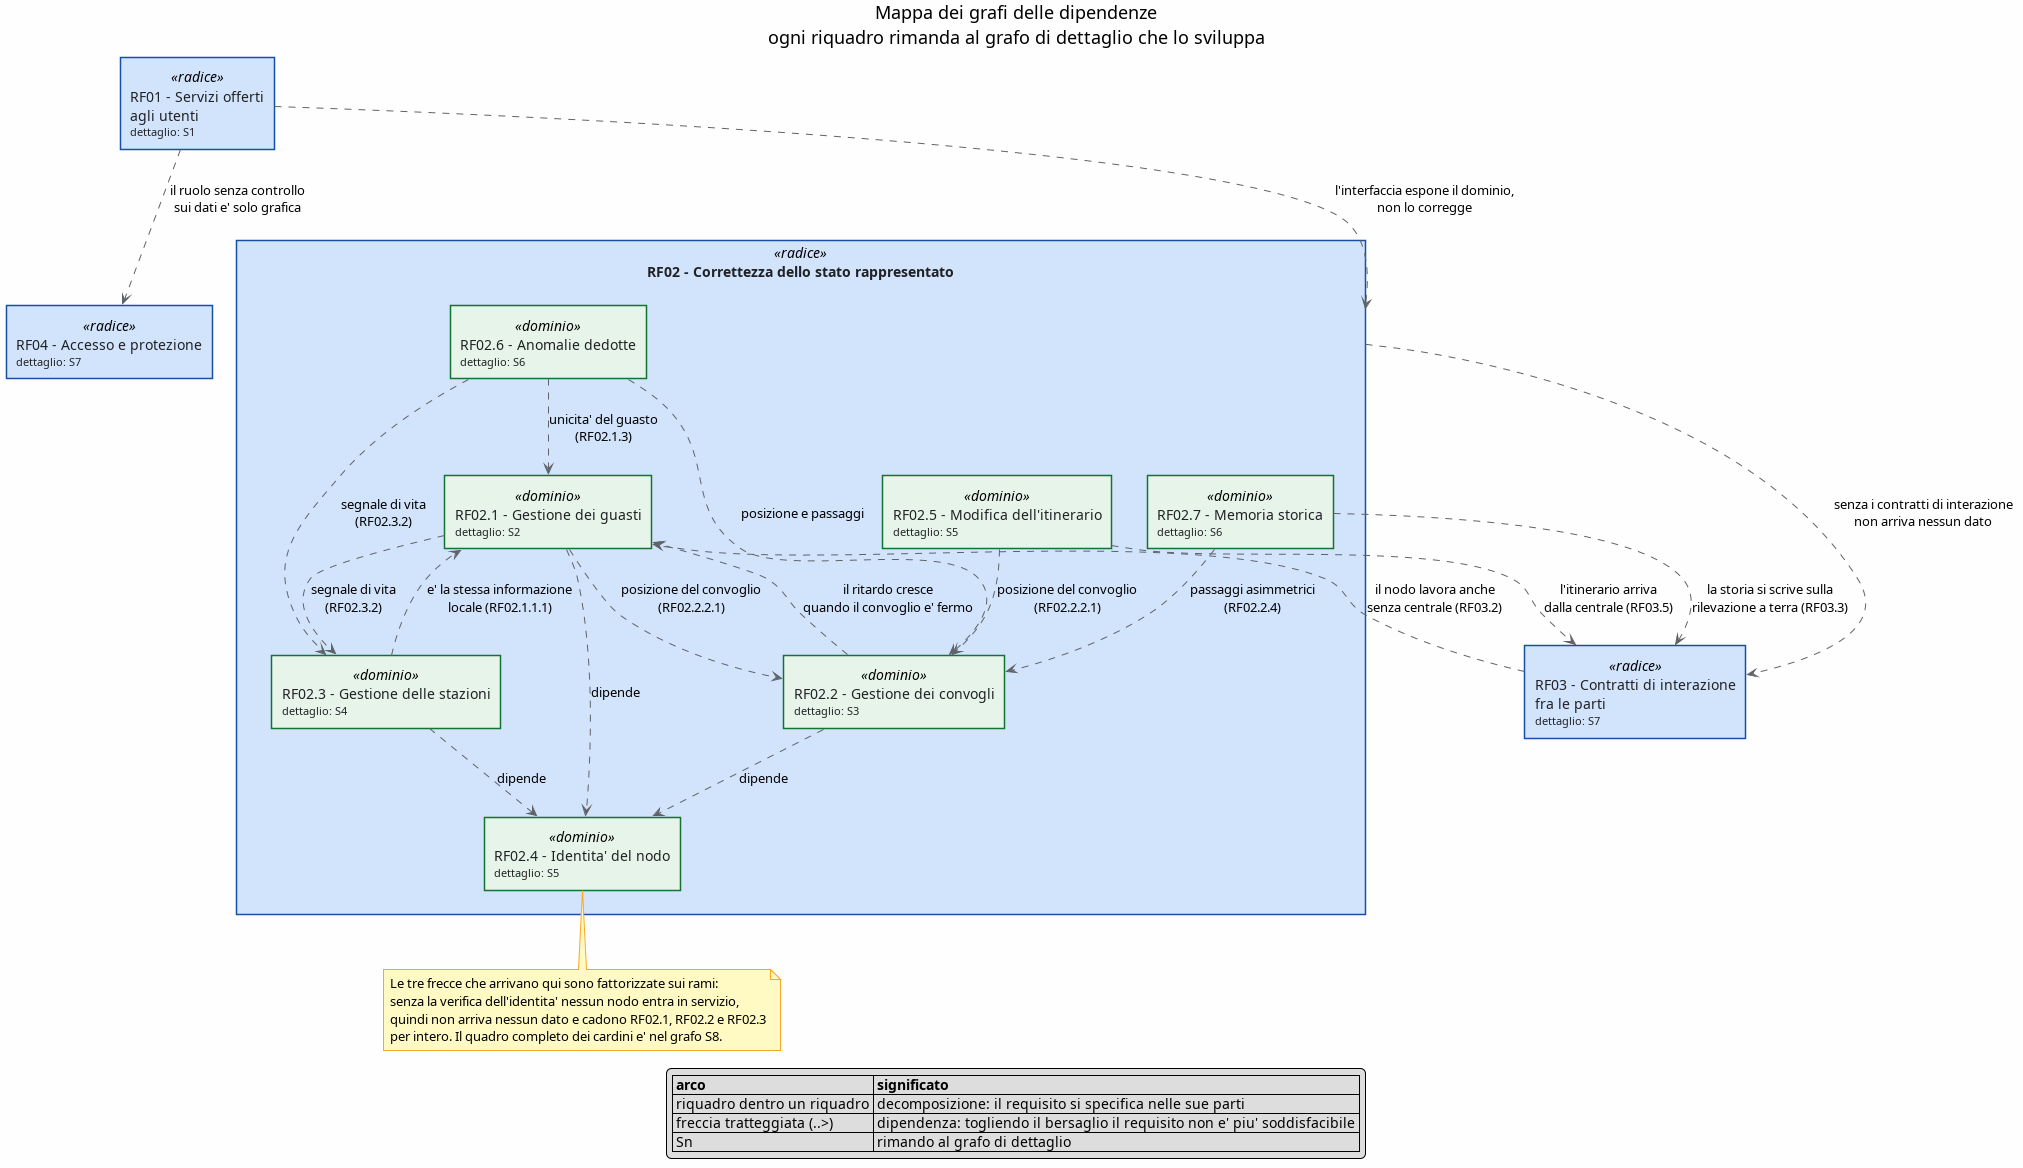
\includegraphics[width=.9\linewidth]{rf_grafo_mappa.png}
\label{}
\end{center}
\subsection{S1 - RF01, i servizi offerti agli utenti}
\label{sec:orgdf6b54e}

RF01 e' quello che l'utente vede: non aggiunge logica al dominio, la espone. Per questo tutte le sue
frecce escono e nessuna entra, e ogni servizio punta al requisito di dominio che lo rende possibile.

\begin{center}
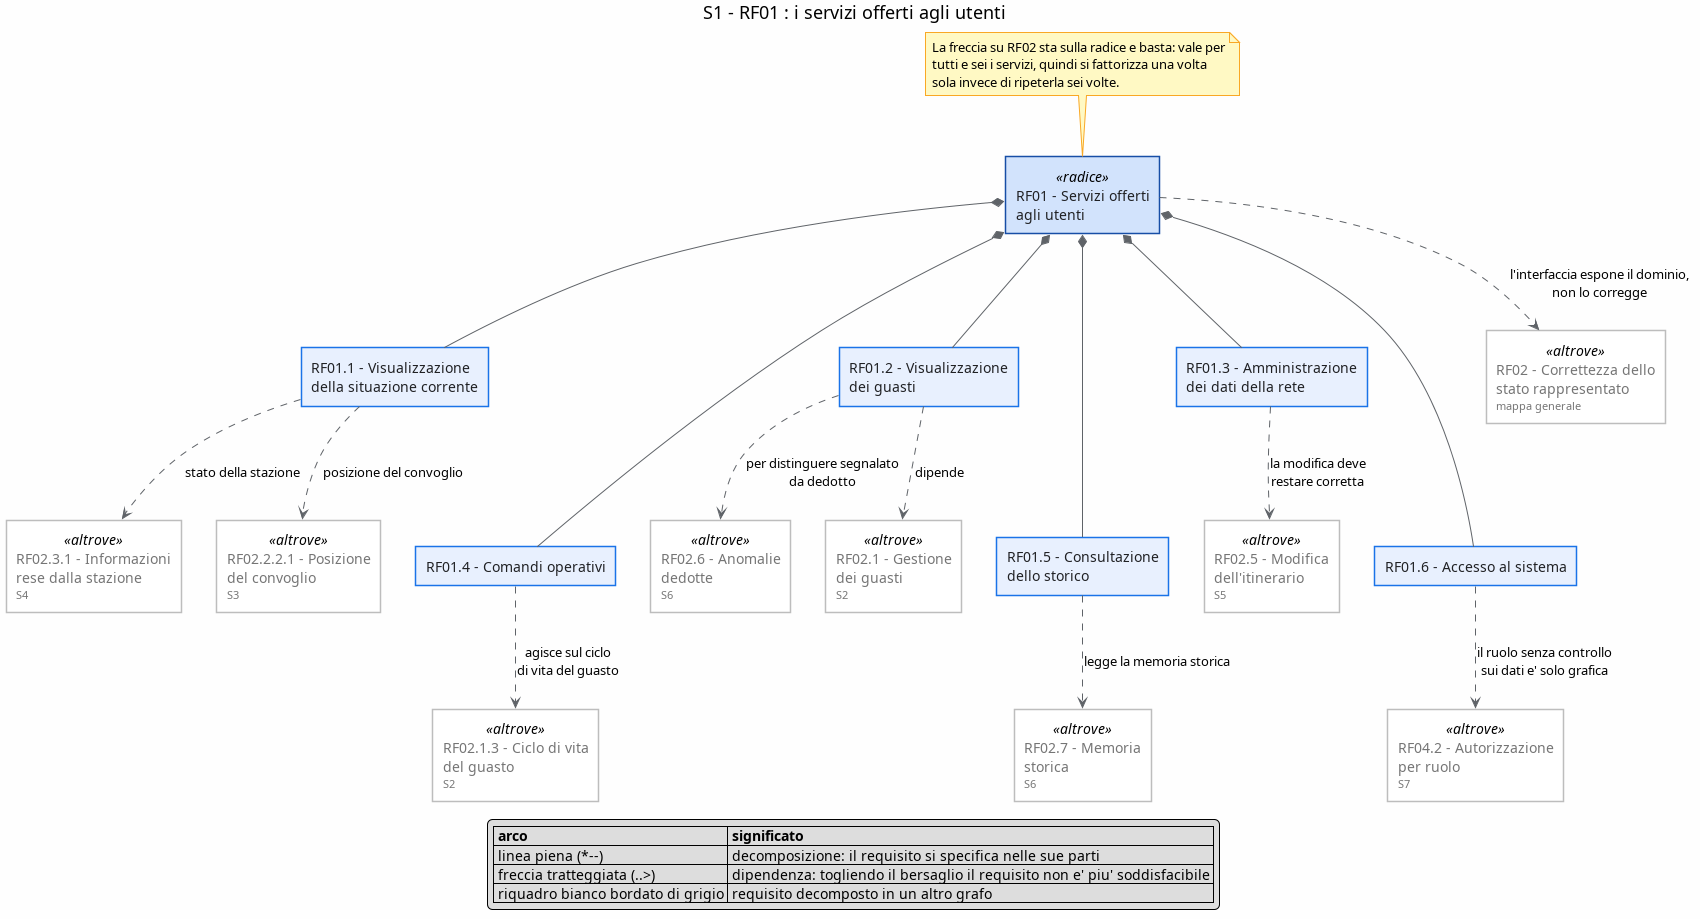
\includegraphics[width=.9\linewidth]{rf_grafo_s1_servizi.png}
\label{}
\end{center}
\subsection{S2 - RF02.1, la gestione dei guasti}
\label{sec:orgc53cde8}

Il guasto segnalato dal campo. Le conseguenze di un guasto sono tutte domande sulla posizione del
convoglio, e la chiusura automatica e' una domanda sul segnale di vita: sono i due cardini che questo
ramo consuma.

\begin{center}
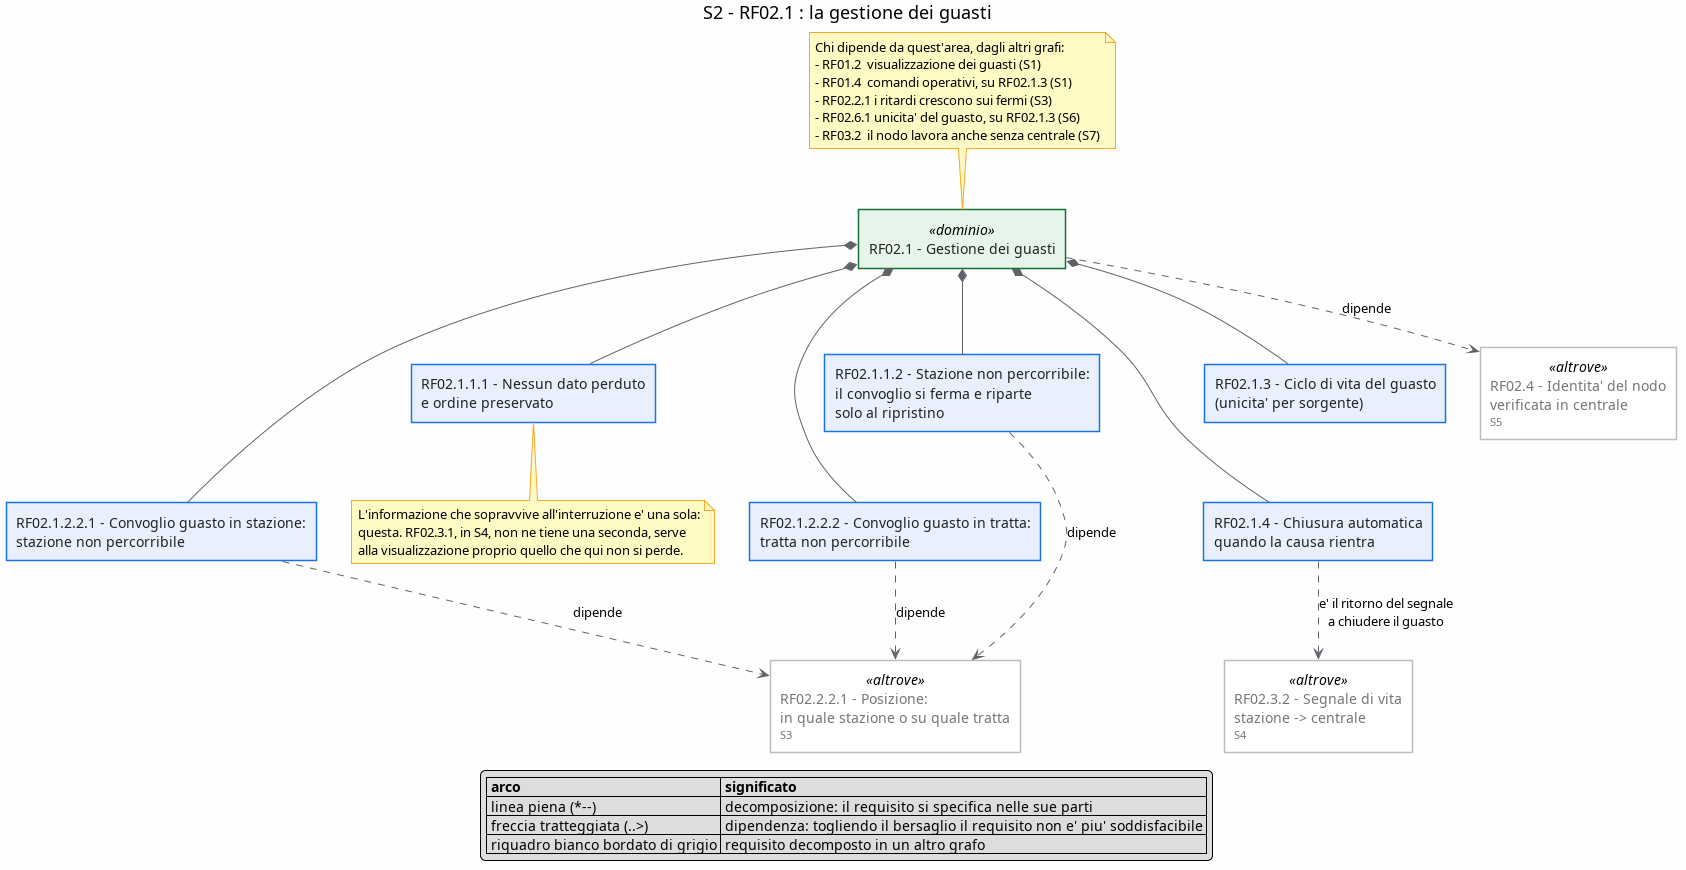
\includegraphics[width=.9\linewidth]{rf_grafo_s2_guasti.png}
\label{}
\end{center}
\subsection{S3 - RF02.2, la gestione dei convogli}
\label{sec:org8603254}

Qui dentro sta RF02.2.2.1, il primo dei tre cardini: la posizione del convoglio. Le frecce che gli
arrivano da fuori sono sei e stanno tutte insieme in S8.

\begin{center}
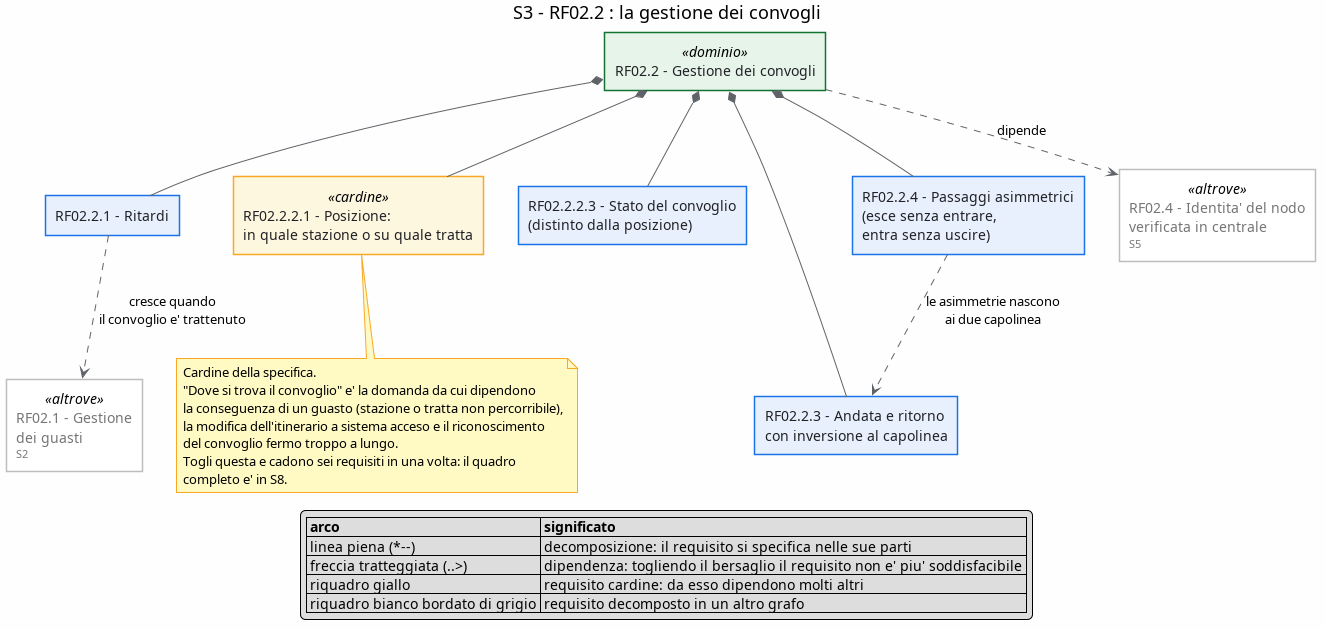
\includegraphics[width=.9\linewidth]{rf_grafo_s3_convogli.png}
\label{}
\end{center}
\subsection{S4 - RF02.3, la gestione delle stazioni}
\label{sec:org5a897bb}

Il secondo cardine e' qui: il segnale di vita della stazione. Il suo valore informativo sta
nell'assenza, ed e' per questo che due requisiti di aree diverse ci si appoggiano.

\begin{center}
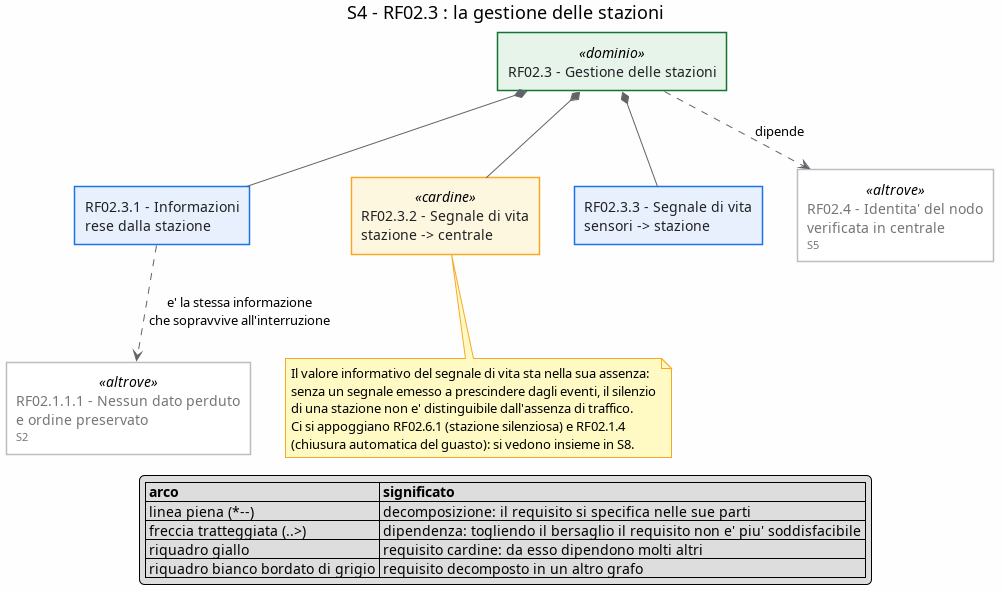
\includegraphics[width=.9\linewidth]{rf_grafo_s4_stazioni.png}
\label{}
\end{center}
\subsection{S5 - RF02.4 e RF02.5, chi entra nel sistema e chi cambia strada}
\label{sec:orge7e9e32}

Due aree piccole ma messe insieme non per comodita': una dice a quali condizioni un nodo entra in
servizio, l'altra a quali condizioni un itinerario puo' cambiare mentre il sistema e' acceso. Sono le
due porte del sistema, una in ingresso e una in corsa.

\begin{center}
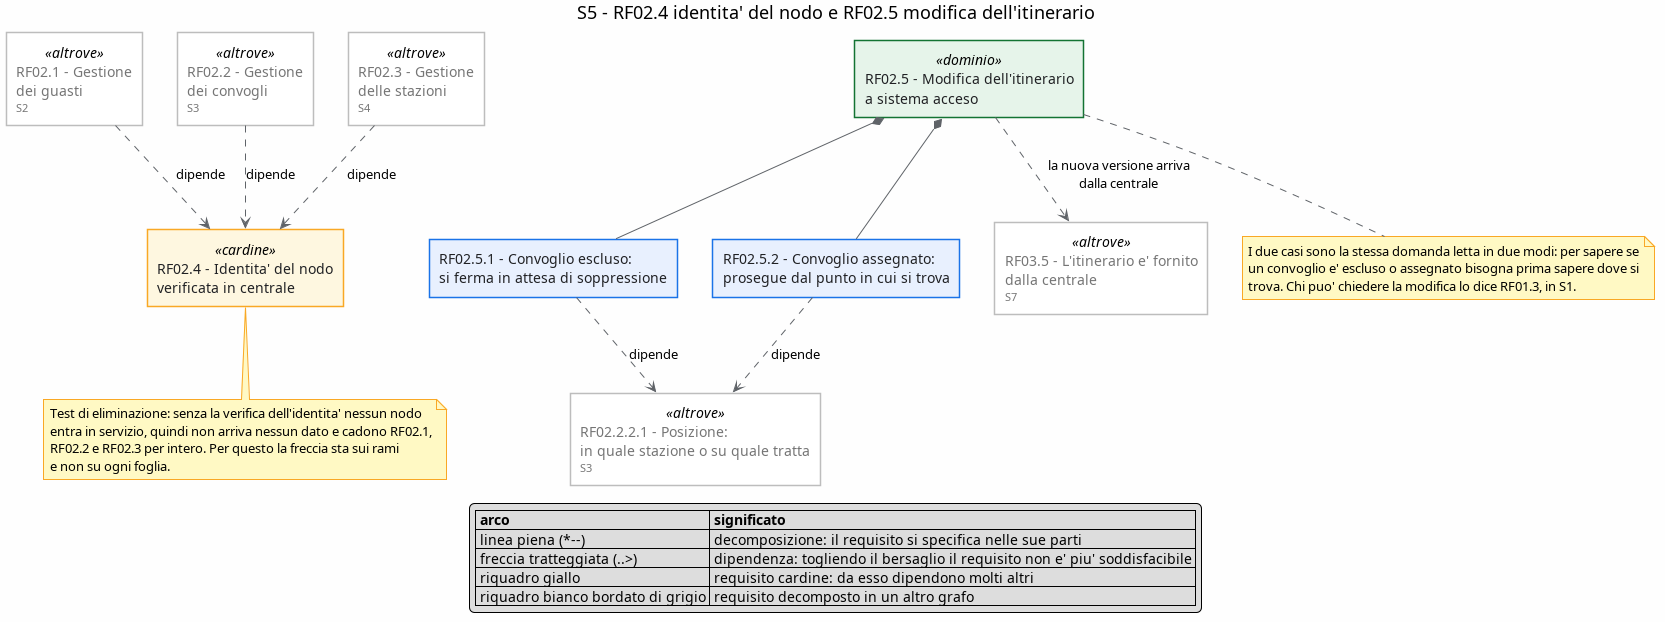
\includegraphics[width=.9\linewidth]{rf_grafo_s5_identita_itinerario.png}
\label{}
\end{center}
\subsection{S6 - RF02.6 e RF02.7, cio' che la centrale deduce e cio' che ricorda}
\label{sec:orgda0c66f}

Le anomalie dedotte non sono segnalate da nessuno: la centrale le ricava da un silenzio o da un
fermo che dura troppo. La memoria storica e' l'altra faccia della stessa cosa: e' quello che resta
quando il momento e' passato.

\begin{center}
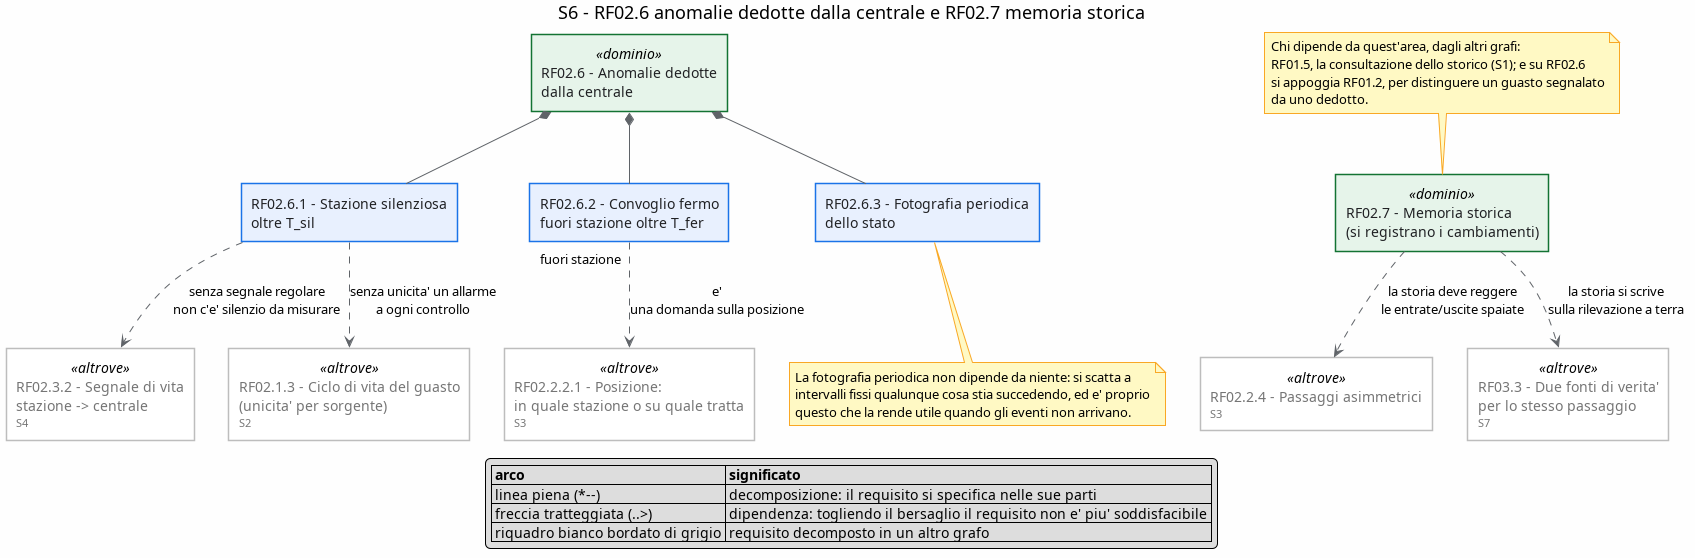
\includegraphics[width=.9\linewidth]{rf_grafo_s6_anomalie_storia.png}
\label{}
\end{center}
\subsection{S7 - RF03 e RF04, i contratti fra le parti e l'accesso}
\label{sec:org895fa2b}

Queste due radici non si vedono da nessuna schermata, ma stanno sotto tutto il resto: RF03 dice a
quali condizioni le parti si parlano, RF04 a quali condizioni qualcuno puo' guardare e toccare.

\begin{center}
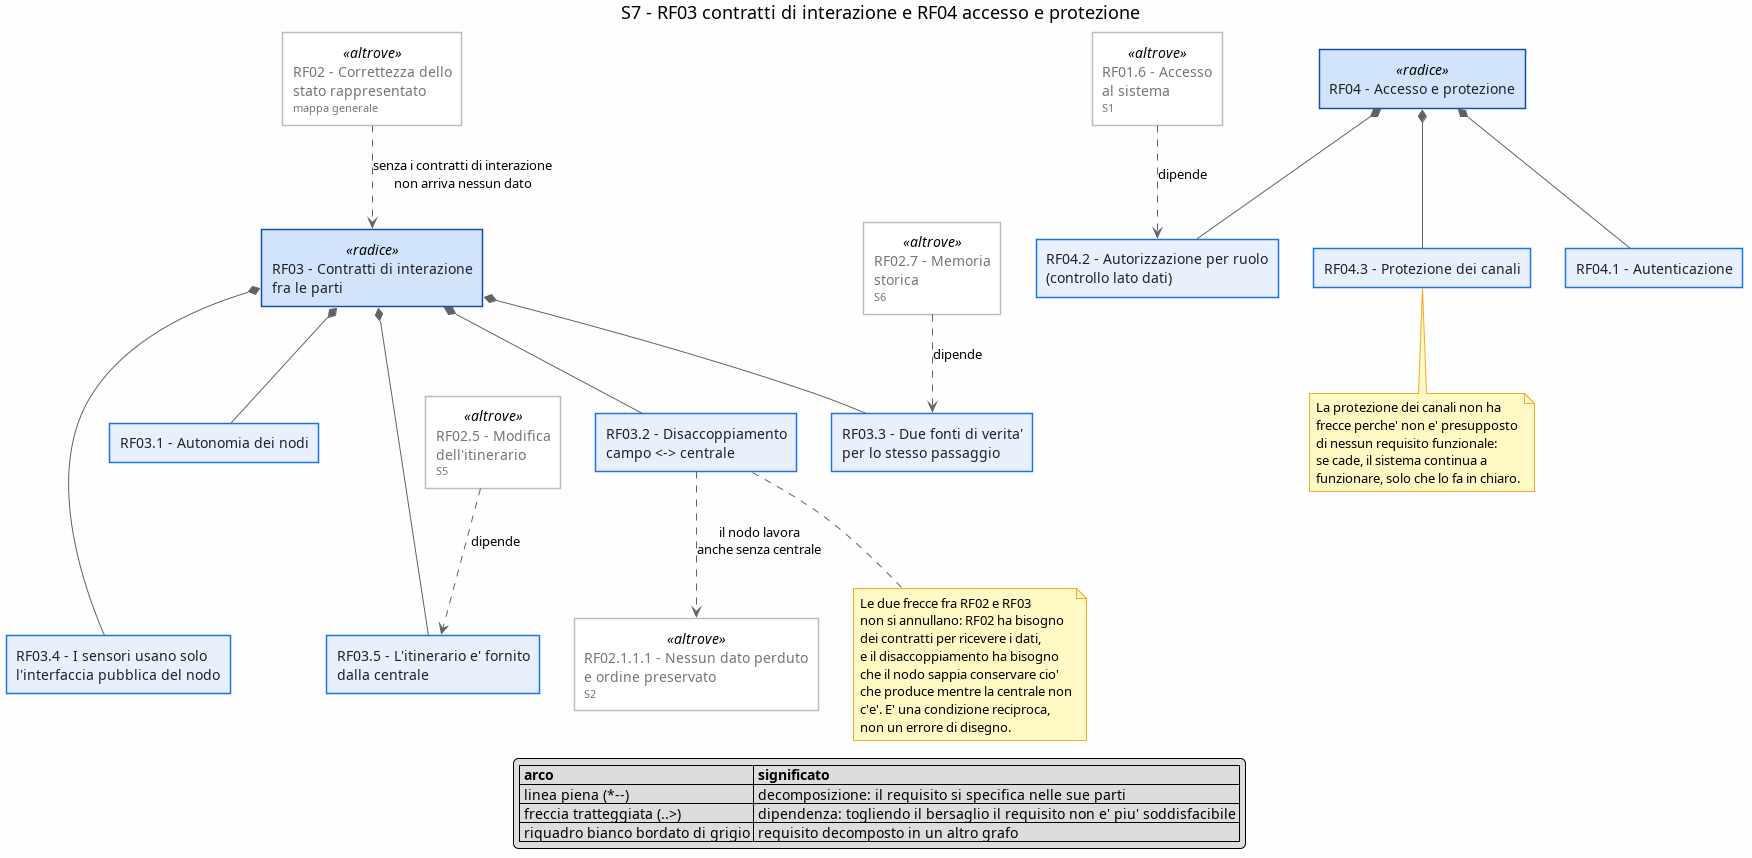
\includegraphics[width=.9\linewidth]{rf_grafo_s7_contratti_accesso.png}
\label{}
\end{center}
\subsection{S8 - i tre cardini}
\label{sec:orgfaaa1f8}

Qui non c'e' nessun arco di decomposizione: ci sono solo i tre requisiti cardine e tutto quello che
cade insieme a loro. E' il grafo da guardare per il test di eliminazione, cioe' per rispondere alla
domanda ``se tolgo questo, che cosa non e' piu' soddisfacibile?''.

\begin{center}
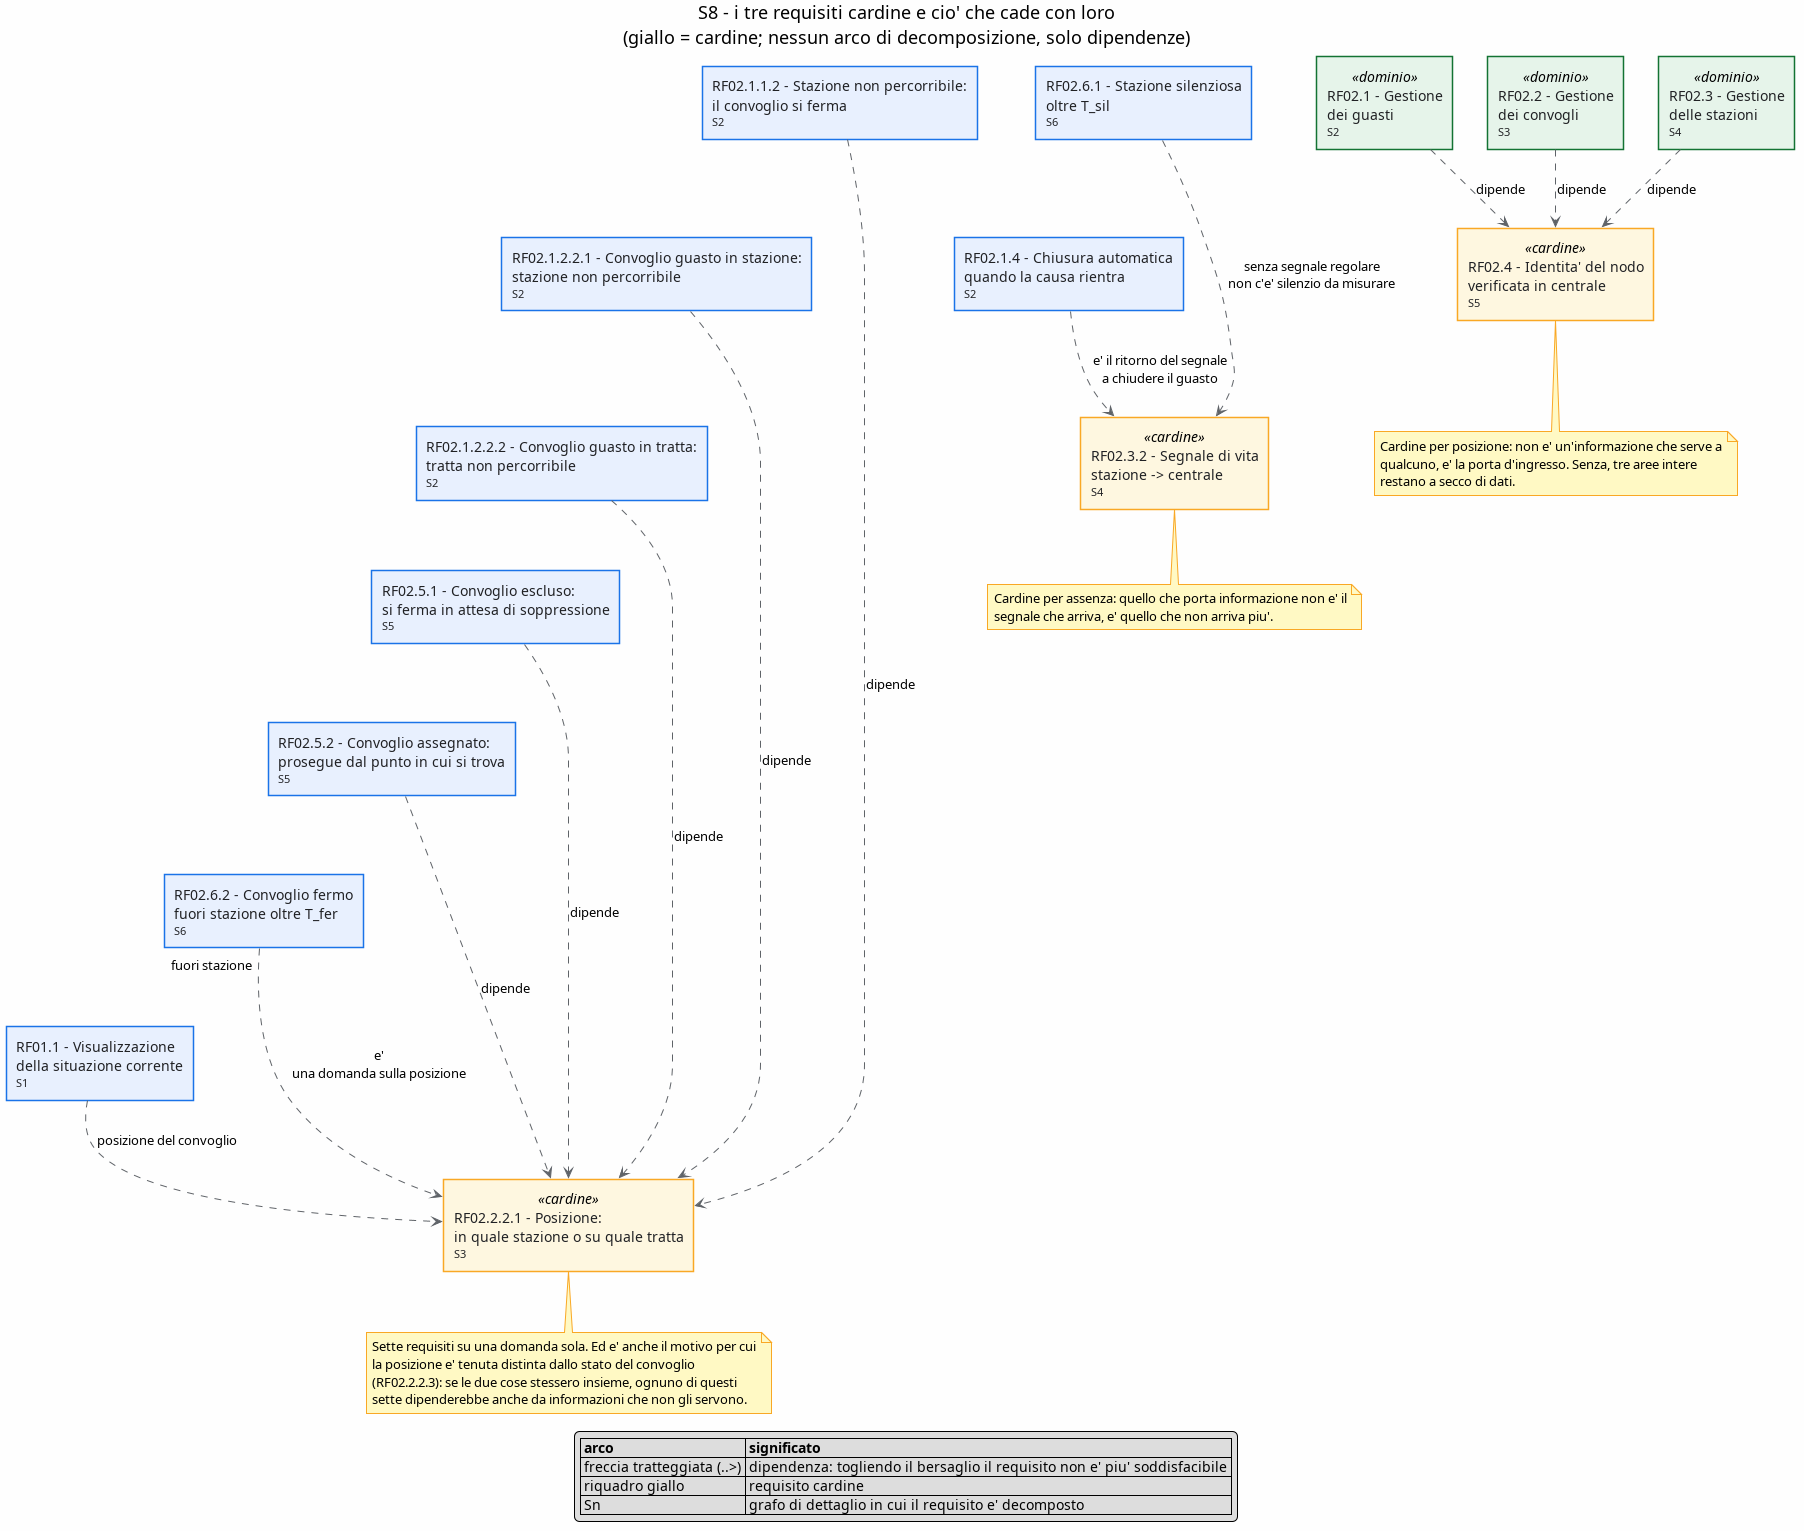
\includegraphics[width=.9\linewidth]{rf_grafo_s8_cardini.png}
\label{}
\end{center}
\end{document}
